\chapter{机器学习}

\originalpage{298}{283}
处理大量和复杂的数据是现代物理学研究中一个非常重要的特征。同时，随着计算物理方法本身的复杂度越来越高，计算过程本身也是一种需要处理大量数据的过程。在这方面，近些年在计算物理中发展最快的一类方法就是机器学习方法。机器学习方法种类繁杂，广泛地涉及物理学的各个分支。本章选取若干有代表性的算法和模型，尝试对若干机器学习方法的主要思想进行简要介绍。

机器学习中常见的类型可以归为监督式学习、非监督式学习和强化学习。监督式学习是基于已经被标记结果的数据对模型进行训练。非监督式学习是在没有标记的数据集用以训练的情况下进行的机器学习。强化学习则更加关注模型和数据之间的交互，利用反馈机制来优化模型。实际上，这种分类也并非严格，在一些复杂的物理问题中，这些方法常常被混合使用。

在通过机器学习获得有效的训练模型后，物理学的研究主要可以分为两类任务：一类是参数估计任务，比如模型中的某个或者某些参数是具有特定意义的物理参数，这时候模型训练过程就是找到这个最优参数的过程。这种任务在传统的回归模型中最为典型，因为传统的解析模型常常是根据已有的物理理论公式得到的。第二类任务是预测任务，也就是用训练得到的模型来预测新的自变量所对应的输出结果。与解析模型相比，机器学习模型更像一个“黑盒子”，其中的参数的物理意义并不明确，反而是预测新的数据更加实用。尤其是当某一类数据的获得成本比较高时，机器学习模型能够成为各类数值研究的重要支撑。

以经典系统的力场模型的构建为例，力场决定了经典体系中粒子间的相互作用，所以力场构造就是要找到一个体系粒子位置 $(r)$ 和能量 $(V)$ 或力 $(F)$ 之间的映射关系 $f_\theta:r\to V;F$。在过去的研究中，相互作用的形式往往是通过经验力场给定的，其普适性无法保证。而我们知道，如果应用 Born--Oppenheimer 近似，把体系的电子和原子核进行变量分离，就可以用第一性原理电子结构计算来获得体系原子间的相互作用。计算得到的相互作用数据就是一组已标记的数据，它包括了给定的粒子坐标和对应的势能，以及势能对原子位置的梯度（即受力）。因此，从第一性原理计算数据出发训练力场模型就恰好是一个类似于回归问题的监督式学习问题。

求解量子多体问题的目标实际上也是建立量子粒子的微观状态到其宏观量子态的映射。这种映射看起来会比经典情形更加难以建立，但是原则上也可以通过机器学习模型来建立。如果在构造模型的时候保持体系的变分性，那么就可以将体系的能量作为损失函数来对网络参数进行优化。这时候网络优化过程就是机器学习中的训练过程，它不再依赖于已知的训练数据，是典型的非监督式学习。

\originalpage{299}{284}
\section{模型回归：监督式学习}

\subsection{回归问题}
我们先以回归问题为例来对机器学习的基础理论进行简要的梳理。记物理实验或观测的自变量为 $x=\{x_1,x_2,\ldots,x_N\}$，共有 $N$ 个影响测量的因素，对应的因变量为测量物理量 $y$。物理的测量（包括实验和数值检验）就是得到了很多组对应的数据集。已知或者待发现的物理规律都可以简化为一个从自变量到因变量的映射关系，$f_\theta:x\to y$。这个映射关系依赖于一组参数 $\theta$。这个映射关系也可以叫作模型，机器学习中的一类问题就是为了能够得到这个模型，从而用于预测新的数据。而传统上，这类问题就叫作回归问题。

在 3.3 节中我们已经介绍了最小二乘法，也就是通过预测值和已知值之间的方差来得到最优参数 $\theta_{\mathrm{opt}}$：
\begin{equation}
\theta_{\mathrm{opt}}:\min_\theta\sum_i|\epsilon_i|^2
=\min_\theta\sum_i|y_i-f_\theta(x_i)|^2.
\tag{8.1.1}
\end{equation}
那里的主要思路是将参数的改变量记为 $\delta\theta=\theta-\theta_0$，将 $f_\theta(x_i)$ 根据其梯度进行一阶展开，然后将上述优化问题转化为线性方程组的求解问题。

如果用机器学习的语言再来看回归问题，则可以把最小二乘法拟合看成一种监督式学习。为此，我们可以从贝叶斯统计理论的角度来理解该过程。根据贝叶斯定理，数据和参数都满足特定的统计分布，且满足如下关系式：
\begin{equation}
P(\theta|X)=\frac{P(\theta)P(X|\theta)}{P(X)},
\tag{8.1.2}
\end{equation}
其中 $P(X)$ 是观测数据的概率分布。参数 $\theta$ 本征的分布（不考虑任何已知数据的情况）称为模型的先验分布（prior），记为 $P(\theta)$。$P(\theta|X)$ 是贝叶斯后验分布（posterior），它描述的是考虑测量数据 $X$ 以后对于参数 $\theta$ 的理解。$P(X|\theta)$ 是似然函数（likelihood），它是指在给定的模型参数下测量得到数据 $X$ 的条件概率。

观测数据的分布 $P(X)$ 可以进一步分解为所有可能的参数 $\theta'$ 所预测的分布的平均分布：
\begin{equation}
P(X)=\int P(X|\theta')P(\theta')\,d\theta'.
\tag{8.1.3}
\end{equation}

\originalpage{300}{285}
对于每个给定的模型参数 $\theta'$，测量得到数据 $X$ 的条件概率是似然函数 $P(X|\theta')$。而数据 $X$ 是这些所有可能的模型参数给出的预测按照参数自身的概率分布的权重积分得到的，该式说明在贝叶斯统计理论的逻辑下，即使是已知的数据，依然可以用统计分布来理解。

按照同样的逻辑，贝叶斯公式也描述了测量过程中对于模型参数认知的修正。假定 $X$ 是一组已经测量的数据，$D$ 是一组新的测量数据，用 $DX$ 记更新后的所有数据，于是
\begin{equation}
P(\theta|DX)=\frac{P(\theta)P(DX|\theta)}{P(DX)},
\tag{8.1.4}
\end{equation}
$P(DX|\theta)$ 表示给定模型参数 $\theta$ 时观测到数据集 $DX$ 的条件概率，$P(\theta|DX)$ 表示考虑了数据 $DX$ 以后对模型参数 $\theta$ 的理解。应用概率分布的乘法法则，$P(DX|\theta)=P(D|\theta)P(X|D\theta)$，其中左式第一项为给定模型参数 $\theta$ 测量 $D$ 的条件概率 $P(D|\theta)$，右式第二项为给定模型参数 $\theta$ 且已经获得 $D$ 测量时候再测量 $X$ 得到的概率 $P(X|D\theta)$。

利用条件概率的定义，可以将上式进一步展开得
\begin{equation}
P(\theta|DX)=\frac{P(\theta)P(D|\theta)P(X|D\theta)}{P(DX)}
=P(\theta|X)\frac{P(D|\theta X)}{P(D|X)}.
\tag{8.1.5}
\end{equation}
上式中左侧 $P(\theta|DX)$ 代表考虑新的数据以后预测的模型参数，右式第一项为只考虑原数据 $X$ 的情况下对模型参数的预测，$P(D|\theta X)/P(D|X)$ 就相当于新的数据对于原数据预测的分布的修正。其中，$P(D|X)$ 表示给定数据 $X$ 的情况下生成新的数据 $D$ 的概率，而分子项 $P(D|\theta X)$ 表示给定这组数据 $X$ 不变且给定参数 $\theta$ 时数据 $D$ 生成的概率。

总之，贝叶斯统计为我们提供了一个直观的从测量数据中获得模型的方法论。其中，似然函数 $P(X|\theta)$ 给出了关于模型优劣的关键信息。我们可以把 $P(X|\theta)$ 理解为 $P(\mathrm{Data}|\mathrm{Model})$，也就是在一个给定的模型下获得数据的条件概率分布，如果一个模型预测已知存在的数据具有很小的概率，那么直观上就可以认为这个模型比较糟糕。可以证明最好的模型正是似然函数取最大的情况。所以模型的优化算法可以从似然函数的最大化推导出来，一般是通过取似然函数的对数的相反数，从而转化为极小值问题来计算。

以最小二乘法拟合为例，考虑数据 $\{x_i,y_i\}$，$i=1,\ldots,N$，回归模型具有 $M$ 个参数，$\theta_1,\ldots,\theta_M$，$y(x)=y(x|\theta_1,\ldots,\theta_M)$。假设测量数据是独立的，且它们符合高斯分布以及统一的标准差 $\sigma$，可以得到似然函数正比于所有数据高斯分布的乘积：
\begin{equation}
P(\mathrm{Data}|\mathrm{Model})\propto\prod_{i=1}^{N}\exp\left[-\frac12\left(\frac{y_i-y(x_i|\theta_1,\ldots,\theta_M)}{\sigma}\right)^2\right].
\tag{8.1.6}
\end{equation}

\originalpage{301}{286}
对它取极大值，可以得到
\begin{equation}
\max P(\mathrm{Data}|\mathrm{Model})\Longleftrightarrow
\min\sum_{i=1}^{N}\bigl(y_i-y(x_i|\theta_1,\ldots,\theta_M)\bigr)^2,
\tag{8.1.7}
\end{equation}
这就是最小二乘法的原始表达式。

进一步考虑线性回归，将拟合函数写为 $y=\theta x+\epsilon$（注意，这里的 $\theta$ 表示由多个参数影响得到的系数，取似然函数对数的极大值时的参数
\begin{equation}
\theta_{\mathrm{opt}}:\max_\theta l(\theta),
\tag{8.1.8}
\end{equation}
其中 $l(\theta)=\ln p(y|x,\theta)$。

对于独立数据，且假设数据满足一维高斯分布 (8.1.6) 式的情况下，
\begin{equation}
l(\theta)=-\frac1{2\sigma^2}\sum_{i=1}^{N}(y_i-\theta x_i)^2-\frac N2\ln(2\pi\sigma^2),
\tag{8.1.9}
\end{equation}
其中 $N$ 为拟合数据的数量。

进一步，假设参数 $\theta$ 也满足一个高斯先验分布，根据贝叶斯规则，$p(\theta|D)\propto p(D|\theta)p(\theta)$，可以把对数似然函数分解成两项之和，因此最优参数的表达式为
\begin{equation}
\theta_{\mathrm{opt}}:\max_\theta\left[-\frac1{2\sigma^2}\sum_{i=1}^{N}(y_i-\theta x_i)^2-\frac1{2\tau^2}\theta^2\right],
\tag{8.1.10}
\end{equation}
其中 $\tau$ 为参数 $\theta$ 的标准差。如果取一个超参数 $\lambda=\sigma^2/\tau^2$，则正好对应为里奇（Ridge）正则化的线性回归。

总地来说，基于贝叶斯统计，数据点和参数都可以假设为满足某个分布，回归模型中的分布假设对应不同的拟合公式。同样的道理，对于一组特定的拟合公式，总是可以根据贝叶斯统计尝试反推得到其可能的统计假设，只是这个假设并不一定唯一。

\subsection{机器学习模型误差}
在机器学习中不可避免地要用统计的语言讨论机器学习的有效性，也就要讨论模型的误差。为了能够定量评估模型的预测能力，在监督式机器学习中一般会将已知的数据分为两组：一组称为训练集，记为 $\{X_{\mathrm{train}};Y_{\mathrm{train}}\}$，另一组称为测试集，记为 $\{X_{\mathrm{test}};Y_{\mathrm{test}}\}$。在训练完成时得到的误差称为训练误差 $E_{\mathrm{train}}=C(Y_{\mathrm{train}},f_{\theta_{\mathrm{opt}}}(X_{\mathrm{train}}))$，也叫作样本内误差。测试集的误差评估叫作测试误差 $E_{\mathrm{test}}=C(Y_{\mathrm{test}},f_{\theta_{\mathrm{opt}}}(X_{\mathrm{test}}))$，也叫作样本外误差。要获得一个好的机器学习模型，就要同时让其训练误差和测试误差满足要求。测试误差与训练误差之间的差别代表了模型的泛化能力，泛化能力差意味着测试误差更加偏离训练误差。

\originalpage{302}{287}
而误差又可以分为两类。一类是系统误差，反映模型的预测值对于真实值的偏离程度。另一类是模型预测值的统计误差，反映模型预测的不确定度。要减小系统误差，一般需要增加机器学习模型的复杂度，但是模型复杂度的增加使得数据量相对变小，所以模型的训练会不充分，导致统计误差变大。图 8.1 展示了在数据量不变的情况下误差随着模型复杂度的变化关系的一般规律。随着模型复杂度的增加，模型训练的系统误差会下降，与此同时统计误差升高。一般来说，考虑测试误差随着模型复杂度的关系，存在一个最佳平衡位置，这时对应于测试误差可以取到最小值的情况。

\begin{figure}[htbp]
\centering
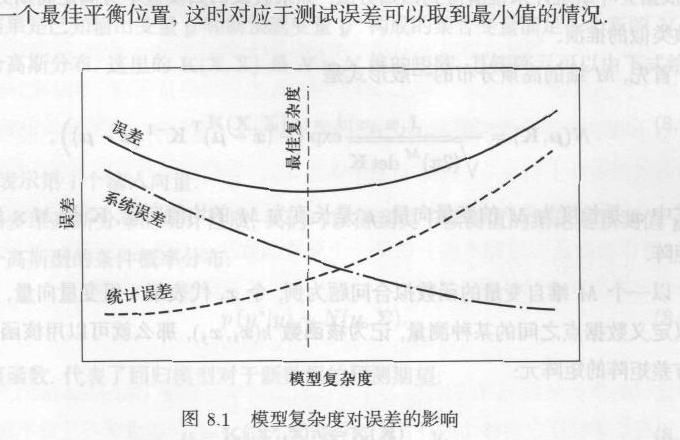
\includegraphics[width=0.70\linewidth]{figures/fig8_1_bias_variance.png}
\caption{模型复杂度对误差的影响}
\label{fig:model-complexity-error}
\end{figure}

当模型复杂度小于最佳值的时候，模型的统计误差比较小，但是系统误差比较大，这种情况称为模型的欠拟合，对应的模型为低方差高偏差模型。反之，当模型复杂度大于最佳平衡值时，模型为高方差低偏差模型，也就是系统误差比较小，但是统计误差比较大，这种情况也叫作模型的过拟合。图 8.2 展示了多项式拟合中出现的过拟合和欠拟合情况的直观图像。

\begin{figure}[htbp]
\centering
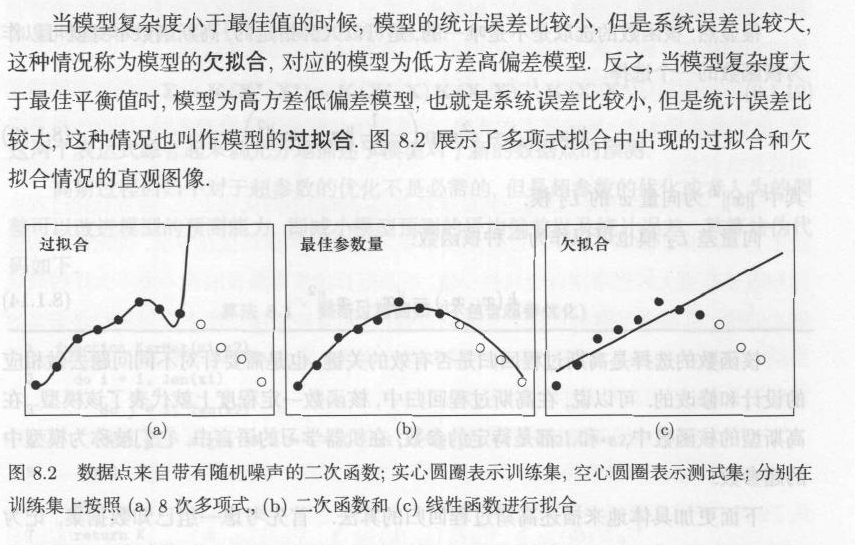
\includegraphics[width=0.94\linewidth]{figures/fig8_2_over_under_fit.png}
\caption{数据点来自带有随机噪声的二次函数；实心圆圈表示训练集，空心圆圈表示测试集；分别在训练集上按照 (a) 8 次多项式，(b) 二次函数和 (c) 线性函数进行拟合}
\label{fig:over-under-fit}
\end{figure}

\originalpage{303}{288}
\subsection{高斯过程回归}
上面这种传统的回归方法一般需要假定一个显式形式的回归函数。实际上，机器学习的理论可以包括更广义的基于统计过程的回归模型。一个典型的方法是高斯过程回归。高斯过程是一种基于高斯分布的随机过程。高斯过程回归的基本假设是回归模型本身满足高斯分布。上面我们已经介绍了如何从数据或者模型参数满足统计分布出发，根据贝叶斯统计来推演得到回归方法。如果假设回归模型本身满足高斯分布，也可做类似的推演。

首先，$M$ 维的高斯分布的一般形式是
\begin{equation}
N(\bm\mu,\mathbf K)=\frac1{\sqrt{(2\pi)^M\det\mathbf K}}\exp\left[-\frac12(\mathbf x-\bm\mu)^\mathrm T\mathbf K^{-1}(\mathbf x-\bm\mu)\right],
\tag{8.1.11}
\end{equation}
上式中 $\mathbf x$ 是长度为 $M$ 的变量向量，$\bm\mu$ 是长度为 $M$ 的均值向量，$\mathbf K$ 是 $M\times M$ 的协方差矩阵。\jiaokan{印本式 (8.1.11) 的指数缺少标准多元高斯分布中的因子 $1/2$。对协方差矩阵 $\mathbf K$，正确指数为 $-\tfrac12(\mathbf x-\bm\mu)^\mathrm T\mathbf K^{-1}(\mathbf x-\bm\mu)$。}

以一个 $M$ 维自变量的函数拟合问题为例，令 $x_i$ 代表第 $i$ 组变量向量，如果我们可以定义数据点之间的某种测量，记为核函数 $k(x_i,x_j)$，那么就可以用核函数来构造协方差矩阵的矩阵元：
\begin{equation}
(\mathbf K)_{ij}=k(x_i,x_j).
\tag{8.1.12}
\end{equation}
很显然，核函数的选取是不是唯一的，是可以人为指定的，高斯函数本身就可以作核函数的一个选择：
\begin{equation}
k(x_i,x_j)=s^2\exp\left(-\frac1{2l^2}\|x_i-x_j\|^2\right),
\tag{8.1.13}
\end{equation}
其中 $\|x\|^2$ 为向量 $x$ 的 $L_2$ 模。

向量内积也可以作为一种简单的核函数：
\begin{equation}
k(x_i,x_j)=x_i^{\mathrm T}x_j.
\tag{8.1.14}
\end{equation}
\jiaokan{印本式 (8.1.14) 写作 $k(x_i,x_j)=\|x_i-x_j\|^2$，并称其可直接作为高斯过程协方差核。平方欧氏距离一般不是半正定核，不能直接作为协方差函数；这里改为最基本的线性核 $x_i^{\mathrm T}x_j$。距离本身仍可用于构造其他合法核，例如式 (8.1.13) 的平方指数核。}
核函数的选择是高斯过程回归是否有效的关键，也是需要针对不同问题去做相应的设计和修改的。可以说，在高斯过程回归中，核函数一定程度上就代表了该模型。在高斯型的核函数中，$s$ 和 $l$ 都是待定的参数，在机器学习的语言中，它们被称为模型中的超参数。

下面更加具体地来描述高斯过程回归的算法。首先考虑一组已知数据集，记为 $D:\{\mathbf X,\mathbf y\}$。$\mathbf X$ 为 $M\times N$ 维的数据，$M$ 是自变量的维度，$N$ 是已知数据集中的数据点数。令该回归模型预测的新数据为 $D^*:\{\mathbf X^*,\mathbf y^*\}$，$\mathbf X^*$ 是 $M\times N^*$ 维的数据，$\mathbf y^*$ 是长度为 $N^*$ 的向量，$N^*$ 也代表了预测的数据点的数目。

\originalpage{304}{289}
根据前面的介绍，从数据满足高斯分布这一假设出发，可以把已知数据和新数据组合构成一个联合高斯分布：
\begin{equation}
\binom{\mathbf y^*}{\mathbf y}\sim N\left(0,
\begin{pmatrix}
\mathbf K(\mathbf X^*,\mathbf X^*)&\mathbf K(\mathbf X^*,\mathbf X)\\
\mathbf K(\mathbf X,\mathbf X^*)&\mathbf K(\mathbf X,\mathbf X)
\end{pmatrix}\right).
\tag{8.1.15}
\end{equation}
直观的结果是已知输出变量 $\mathbf y$ 和新预测变量 $\mathbf y^*$ 构成的集合变量满足一个新的 $N+N^*$ 维的联合高斯分布。这里的 $\mathbf K(\mathbf X,\mathbf X)$ 是 $N\times N$ 维的矩阵，其矩阵元可以由下式给出：
\begin{equation}
\mathbf K(\mathbf X,\mathbf X)_{ij}=k(x_i,x_j),
\tag{8.1.16}
\end{equation}
其中 $x_i$ 表示第 $i$ 个输入向量。

根据多维高斯分布的统计性质，我们可以得到关于预测值的结论是预测值 $\mathbf y^*$ 也满足一个高斯型的条件概率分布：
\begin{equation}
p(\mathbf y^*|\mathbf y)\sim N(\bm\mu,\bm\Sigma).
\tag{8.1.17}
\end{equation}
$\bm\mu$ 是均值函数，代表了回归模型对于新数据的预测期望：
\begin{equation}
\bm\mu=\mathbf K(\mathbf X^*,\mathbf X)\mathbf K(\mathbf X,\mathbf X)^{-1}\mathbf y,
\tag{8.1.18}
\end{equation}
$\bm\Sigma$ 是对应预测的方差，代表了预测的统计涨落：
\begin{equation}
\bm\Sigma=\mathbf K(\mathbf X^*,\mathbf X^*)-\mathbf K(\mathbf X^*,\mathbf X)\mathbf K(\mathbf X,\mathbf X)^{-1}\mathbf K(\mathbf X,\mathbf X^*).
\tag{8.1.19}
\end{equation}
这两个表达式综合起来就充分地描述了模型对于新的数据点的预测。

高斯过程回归中对于超参数的优化不是必需的，但是超参数的优化或者人为的调整可以改进模型的预测能力，即减小模型预测的平均偏差以及统计误差。其算法伪代码如下。

\begin{algorithmBox}[算法 8.1\quad 高斯过程回归（不包含超参优化）]
\begin{lstlisting}[style=bellacode]
function KerMat(x1,x2)
    do i = 1, len(x1)
        do j = 1, len(x2)
            K(i,j) = sigma ** 2 * exp(-(x1(i)-x2(j)) ** 2 / 2 / l ** 2)
        end
    end
    return K
end

function GPR(x,x0,y0)
    K1 = KerMat(x,x0)
    K2 = KerMat(x0,x0)
    K3 = KerMat(x,x)
    mu = K1.(K2 ** -1).y0
    Sigma = K3 - K1.(K2 ** -1).(K1.T)
    return mu, Sigma
end
\end{lstlisting}
\end{algorithmBox}
\jiaokan{算法 8.1 印本第 4 行将高斯核指数写成了“\texttt{e * (...)}”，这只是 $e$ 与指数的普通乘积，与式 (8.1.13) 不符；此处按核函数定义改为 \texttt{exp(...)}。}

\originalpage{305}{290}
\subsection{机器学习模型的参数优化}
本小节中我们介绍一般的优化机器学习模型中参数的方法。上面已经展示了，机器学习模型实际上就是一个非常复杂的高维函数，我们定义的成本函数（或损失函数）也是一个关于参数 $\theta$ 的高维函数，记为 $E(\theta)$。优化过程就是最小化成本函数 $E(\theta)$ 的过程，所以参数优化过程本质上就是一个高维函数的全局极小值问题。关于函数极值的问题在第四章中已经讨论清楚了，如可以采用基于梯度下降的算法
\begin{equation}
\theta_{t+1}=\theta_t-\eta_t\nabla_\theta E(\theta_t),
\tag{8.1.20}
\end{equation}
其中迭代的步长参数 $\eta_t$ 在机器学习中对应模型的学习速率（learning rate），它控制着迭代过程沿着梯度方向移动的步长。如果步长太大，可能会造成学习过程不稳定，在偏离极值的不同位置之间来回跳动。如果步长太小，可能会导致学习效率比较低，需要很长时间的迭代才能收敛。这些都可以类比一般的函数极值优化过程。

在函数极值优化中还有一类是需要二阶导数信息的牛顿法，对于机器学习模型来说，由于参数量太大，从效率方面考虑，计算高阶导数是要尽量避免的，所以一般不采用这种迭代法。

另外，值得注意的是，这些迭代法求解都是局域极值的优化方法。参数优化过程本质上是全局极小值的优化，不过由于没有稳定而高效的全局优化方法，优化算法的设计初衷是有更大的概率接近全局极小值，不希望算法很容易被陷在一个不太好的局域极小值中。机器学习模型具有非常高的参数维度，直接采用梯度下降等算法是非常容易陷入局域极值点的。因此，机器学习中采用的优化算法是针对参数量巨大的情况所特殊设计的，下面列举其中几种常用的算法：

一种常用的改进是随机梯度下降，它把一批次（batch）的数据分成很多个小的微批次（mini-batch），
\begin{equation}
\nabla_\theta E(\theta_t)=\sum_{i=1}^{N}\nabla_\theta E_i(x_i,\theta_t)\approx\sum_{i\in B_k}\nabla_\theta E_i(x_i,\theta_t),
\tag{8.1.21}
\end{equation}

\originalpage{306}{291}
其中 $E_i(x_i,\theta_t)$ 是每个数据点 $x_i$ 计算得到的成本函数，$B_k$ 代表一个微批次，通常是几十到几百个数据点（设为 $M$），则 $k=1,\ldots,N/M$。迭代中的一步就用 $B_k$ 数据计算得到的梯度进行，而把所有的数据循环一遍，也即 $N/M$ 次微批次的迭代，称为迭代一代（epoch）。在随机梯度下降训练过程中，参数被更新的总次数应该是代的数目乘以微批次的数目。随机梯度优化算法中引入的随机性，可以适当地减弱系统在局域极小值优化的倾向性，通过让优化过程变“慢”而增加其探索到全局极小值的概率。如果将参数空间类比物理系统，它背后蕴含的物理规律是系统处于更低能态的概率要高于其处于更高能态的概率，增加一些随机性还可以避免参数优化过程中被鞍点所束缚住。

在迭代算法中，除了直接的梯度方向的下降，还可以加入上一步的迭代方向的信息，与当前步的迭代做一个混合，这样的算法一般可以使得迭代过程更加稳定，在传统的函数优化方法中的共轭梯度法就是这类算法的一个特例。在机器学习的参数优化中，这样的方法也是很常用的，它的一般形式是
\begin{equation}
\begin{aligned}
\theta_{t+1}&=\theta_t-v_t,\\
v_t&=\gamma v_{t-1}+\eta_t\nabla_\theta E(\theta_t),
\end{aligned}
\tag{8.1.22}
\end{equation}
或者
\begin{equation}
v_t=\gamma v_{t-1}+\eta_t\nabla_\theta E(\theta_t+\gamma v_{t-1}).
\tag{8.1.23}
\end{equation}
后面的这个方法也称为 \rusname{Нестеров} 加速梯度下降（Nesterov accelerated gradient）方法，其中参数 $\gamma$ 是一个可调的参数，一般取 $0\le\gamma\le1$。

另外，还有一些算法引入梯度的平方项进入迭代过程，如著名的 Adam 算法，它的具体过程如下：
\begin{equation}
\begin{aligned}
g_t&=\nabla_\theta E(\theta_t),\\
m_t&=\beta_1m_{t-1}+(1-\beta_1)g_t,\\
s_t&=\beta_2s_{t-1}+(1-\beta_2)g_t^2,\\
m'_t&=\frac{m_t}{1-(\beta_1)^t},\\
s'_t&=\frac{s_t}{1-(\beta_2)^t},\\
\theta_{t+1}&=\theta_t-\eta_t\frac{m'_t}{\sqrt{s'_t+\epsilon}},
\end{aligned}
\tag{8.1.24}
\end{equation}
其中 $\epsilon$ 是为了避免分母出现 0 导致发散而引入的一个很小的常数。

值得注意的是同样的算法对于参数量不同的情况其效果可能是完全不一样的。复杂神经网络的参数优化问题仍然是一个待解决的困难问题。

\originalpage{307}{292}
\section{降维与聚类：非监督式学习}
本节以降维和聚类为例来介绍非监督式机器学习。降维针对的是数据的高维度所带来的复杂性，目标是把无标记的高维数据投影到一个能够反映出该系统关键物理特征的低维空间，可以用于发现新的序参量。而聚类则可以提取复杂数据中的隐藏特征，在对模型进行粗粒化处理等应用中起到帮助。这两类方法有一定的相似性，也经常被联合起来使用。

\subsection{降维}
以统计力学中对微观粒子的研究为例，一个三维空间中的多粒子体系，每个粒子具有三个空间坐标的自由度，那么 $N$ 个粒子就张成了 $3N$ 维的坐标空间。应用前面介绍的蒙特卡洛和分子动力学方法，可以计算模拟得到一系列粒子位置坐标的数据。这些数据反映的是对于坐标空间的采样，我们可以用它们来对物理量进行计算。但是如果面对的问题是揭示物理性质和微观结构之间的构效关系，那么我们还需要找到描述这个对应的体系的结构序参量，把 $f_\theta:\{r_1,\ldots,r_N\}\to y$ 的关系简化为一种新的联系 $f_\theta:\{d_1,d_2,\ldots,d_M\}\to y$，这里 $M$ 一般是尽量小的正整数，比如 1 和 2。传统上，我们基于经验和已有的物理理解来人为地构造这种序参量。本小节将介绍的降维方法就是一类以非监督式学习为主的发现新的序参量的方法。

\subsubsection{主成分分析}
最经典的降维方法之一是主成分分析（principal component analysis, PCA），这是一个相对比较古老的方法。PCA 方法的主要思路是对数据进行正交变换并找到变化最剧烈的方向，从普通的经验上说，变化最剧烈的方向一般是具有最重要信息的方向，而其他变化比较小的正交的方向则可以当作噪声涨落来看待。PCA 方法的原理与效果如图 8.3 所示。

我们下面以经典统计系统为例来具体说明 PCA 的做法。假定 $N$ 个粒子的分布已经由前面章节介绍的蒙特卡洛或者分子动力学方法采样得到。一组模拟采样可以得到 $M$ 个样本，于是可以用一个 $M\times3N$ 的矩阵 $\mathbf X=[x_1,x_2,\ldots,x_M]^\mathrm T$ 来表示所有的数据，每一行代表一组数据，$x_1,x_2,\ldots,x_M$ 代表一个 $3N$ 长度的矢量，描述各个粒子的笛卡儿坐标。以下默认每个特征已经减去其样本均值，即 $\mathbf X$ 已中心化。定义一个 $3N\times3N$ 的协方差矩阵
\begin{equation}
\bm\Sigma(\mathbf X)=\frac1{M-1}\mathbf X^{\mathrm T}\mathbf X,
\tag{8.2.1}
\end{equation}
\jiaokan{印本式 (8.2.1) 的分母写为 $N-1$。这里 $\mathbf X$ 有 $M$ 个样本（行）和 $3N$ 个特征（列），样本协方差的归一化分母应由样本数决定，因此应为 $M-1$；后文式 (8.2.4) 中同一协方差矩阵的归一化也相应采用 $M-1$。}
其中对角项描述的是每一个特征维度的方差，而非对角项则描述了两个不同的特征维度之间的协方差。主成分分析的目的就是对协方差矩阵进行一个线性变换，使得变化

\originalpage{308}{293}
剧烈方向的方差被放大，而变化不剧烈方向被进一步压缩，同时减少不同方向之间的协方差。

\begin{figure}[htbp]
\centering
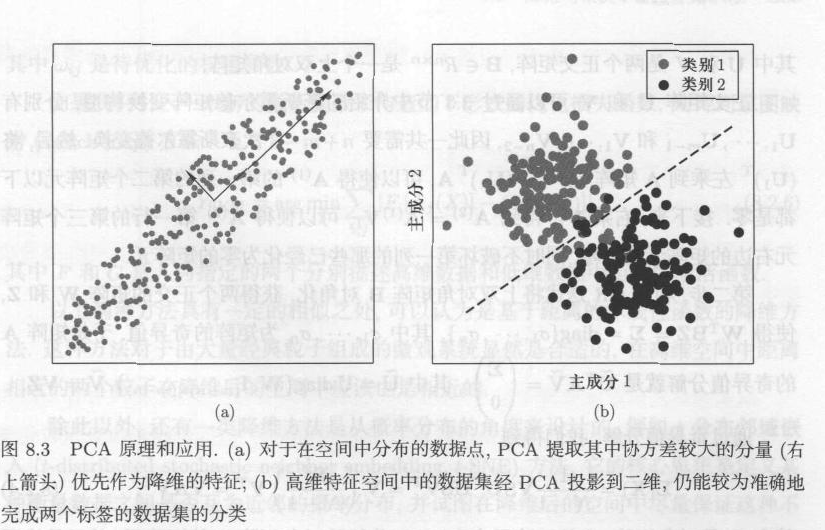
\includegraphics[width=0.92\linewidth]{figures/fig8_3_pca.png}
\caption{PCA 原理和应用。(a) 对于在空间中分布的数据点，PCA 提取其中协方差较大的分量（右上箭头）优先作为降维的特征；(b) 高维特征空间中的数据集经 PCA 投影到二维，仍能较为准确地完成有不同标签的数据集的分类}
\label{fig:pca}
\end{figure}

为此，我们可以对协方差矩阵进行奇异值分解（singular value decomposition, SVD），将矩阵 $\mathbf X$ 分解为 $\mathbf X=\mathbf U\mathbf S\mathbf V^{\mathrm T}$。根据线性代数的知识，对于一个 $m\times n$ 的复矩阵 $\mathbf A\in\mathbb C^{m\times n}$，一定存在两个幺正矩阵 $\mathbf U\in\mathbb C^{m\times m}$ 和 $\mathbf V\in\mathbb C^{n\times n}$ 可以将 $\mathbf A$ 对角化。如果是长方形矩阵，则对角元只包括行列指标相同的矩阵元：
\begin{equation}
\mathbf U^\dagger\mathbf A\mathbf V=\mathbf S=\operatorname{diag}(\sigma_1,\ldots,\sigma_p),\qquad p=\min(m,n),
\tag{8.2.2}
\end{equation}
其中 $\sigma_1\ge\sigma_2\ge\cdots\ge\sigma_p\ge0$ 称为矩阵 $\mathbf A$ 的奇异值。矩阵的非零奇异值实际上是矩阵 $\mathbf A^\dagger\mathbf A$ 的本征值开根号，$\sigma_i(A)=\sqrt{\lambda_i(\mathbf A^\dagger\mathbf A)}$，$\mathbf A^\dagger\mathbf A$ 和 $\mathbf A\mathbf A^\dagger$ 都是厄米的，矩阵 $\mathbf U$ 的列和 $\mathbf V$ 的列分别被称为左奇异矢量和右奇异矢量。如果奇异值的分布满足 $\sigma_1\ge\cdots\ge\sigma_r>\sigma_{r+1}=\cdots=\sigma_p=0$，那么 $\mathbf A$ 的秩为 $r$。它的核 $\ker(\mathbf A)$ 由 $\mathbf V$ 的列矢量 $\{v_{r+1},\ldots,v_n\}$ 张成，而 $\mathbf A$ 的域 $\operatorname{range}(\mathbf A)$ 由 $\mathbf U$ 的列矢量 $\{u_1,\ldots,u_r\}$ 张成。一个矩阵的 SVD 包含了矩阵最重要的信息，虽然两个幺正矩阵不是唯一的，但是实际上几乎是唯一的，只是可能把不同的列进行交换组合而已。

实现矩阵奇异值分解的具体算法之一是 Golub--Kahan--Reinsch 算法。奇异值分解的第一步将矩阵 $\mathbf A$ 变换成如下形式：
\begin{equation}
\mathbf U^{\mathrm T}\mathbf A\mathbf V=\binom{\mathbf B}{0},
\tag{8.2.3}
\end{equation}

\originalpage{309}{294}
其中 $\mathbf U$ 和 $\mathbf V$ 是两个正交矩阵，$\mathbf B\in\mathbb R^{n\times n}$ 是一个上双对角矩阵。

正交矩阵 $\mathbf U$ 和 $\mathbf V$ 可以通过 3.3 节中介绍的 Householder 矩阵变换构造，分别有 $\mathbf U_1,\ldots,\mathbf U_{m-1}$ 和 $\mathbf V_1,\ldots,\mathbf V_{n-2}$，因此一共需要 $n+m-3$ 次 Householder 变换。然后，将 $(\mathbf U_1)^\mathrm T$ 左乘到 $\mathbf A$ 矩阵：$\mathbf A^{(1)}=(\mathbf U_1)^\mathrm T\mathbf A$，可以使得 $\mathbf A^{(1)}$ 的第一列的第二个矩阵元以下都是零。接下来，右乘 $\mathbf V_1$，得到 $\mathbf A^{(2)}=\mathbf A^{(1)}\mathbf V_1$，可以使得 $\mathbf A^{(2)}$ 第一行的第三个矩阵元右边的矩阵元都为零，同时不破坏第一列的那些已经化为零的矩阵元。

第二步，利用 QR 迭代将上双对角矩阵 $\mathbf B$ 对角化，获得两个正交的矩阵 $\mathbf W$ 和 $\mathbf Z$，使得 $\mathbf W^{\mathrm T}\mathbf B\mathbf Z=\bm\Sigma=\operatorname{diag}\{\sigma_1,\ldots,\sigma_n\}$，其中 $\sigma_1,\ldots,\sigma_n$ 为矩阵的奇异值。于是矩阵 $\mathbf A$ 的奇异值分解就是 $\widetilde{\mathbf U}^{\mathrm T}\mathbf A\widetilde{\mathbf V}=\binom{\bm\Sigma}{0}$，其中 $\widetilde{\mathbf U}=\mathbf U\operatorname{diag}\{\mathbf W,\mathbf I_{(m-n)\times(m-n)}\}$，$\widetilde{\mathbf V}=\mathbf V\mathbf Z$。

通过奇异值分解，我们得到
\begin{equation}
\bm\Sigma(\mathbf X)=\frac1{M-1}\mathbf V\mathbf S\mathbf U^{\mathrm T}\mathbf U\mathbf S\mathbf V^{\mathrm T}
=\mathbf V\left(\frac{\mathbf S^2}{M-1}\right)\mathbf V^{\mathrm T}=\mathbf V\bm\Lambda\mathbf V^{\mathrm T},
\tag{8.2.4}
\end{equation}
其中 $\bm\Lambda$ 是对角矩阵，它的矩阵元来自 SVD 分解的对角矩阵 $\mathbf S$ 的矩阵元，并且是按照从大到小排列的。

主成分分析的下一步是将其中最大的 $p$ 个奇异值对应的矢量选出来构成一个投影矩阵 $\mathbf P$。将这个投影矩阵作用到协方差矩阵上就可以得到一个数据的最大的 $p$ 个主成分，即 $\widetilde{\mathbf Y}=\mathbf X\mathbf P$。

\subsubsection{非线性降维方法}
从更一般的角度来理解降维，它可以理解为寻找一种低维数据，使得它与原高维数据的相似性最大化。很显然，相似性是可以有不同定义的，主成分分析中使用的协方差矩阵只是其中之一。这种定义有时候不能有效地实现序参量的分离。因此，在更广泛的机器学习中，人们逐渐针对不同的问题发展出了不同的降维方法。在很多方法中，最终定义的待优化的损失函数不是线性的，因此对应的数值问题不能转化为奇异值分解，而是转化为非线性函数的极值优化问题。

记降维后的数据为 $Y$。定义某个数据分布中两个数据点之间的距离为 $d_{ij}$，$d_{ij}(X)$ 为两个特征维度 $i,j$ 在原数据空间 $X$ 中的距离，$d_{ij}(Y)$ 是数据在降维以后的空间 $Y$ 中的距离。距离 $d_{ij}$ 的定义可以取不同的形式，比如取 $d_{ij}(X)=\|x_i-x_j\|^2=\sum_{m=1}^{M}|x_{mi}-x_{mj}|^2$。取定距离的定义以后，就可以定一个优化目标来寻找满足目标的最佳分布 $Y$。

如果我们取优化的损失函数为距离差的线性组合，就得到多维度标度（multidimensional scaling, MDS）方法：
\begin{equation}
\widetilde Y_{\mathrm{MDS}}=\arg\min_Y\sum_{i<j}\omega_{ij}|d_{ij}(X)-d_{ij}(Y)|,
\tag{8.2.5}
\end{equation}

\originalpage{310}{295}
其中 $\omega_{ij}$ 是待优化的权重参数。

如果我们引入一个新的激活函数来构造如下形式的优化损失函数，则得到草图映射（sketch-map）方法：
\begin{equation}
\widetilde Y_{\mathrm{SKM}}=\arg\min_Y\sum_{i,j}|F[d_{ij}(X)]-G[d_{ij}(Y)]|,
\tag{8.2.6}
\end{equation}
其中 $F$ 和 $G$ 是人为指定的两个分别描述高维数据和低维数据中距离的激活函数。

以上两种方法具有一定的相似之处，可以认为是基于距离的非线性函数的降维方法。这种方法对于由大量经典粒子组成的微观系统显然是合适的，在高维空间中距离相近的两个粒子在降维后的空间中应该也是相近的。

除此以外，还有一类降维方法是从概率分布的角度来设计的，例如 $t$ 分布邻域嵌入（$t$-distributed stochastic neighbor embedding, $t$-SNE）方法，它的核心思想是定义某种衡量数据之间是否互为近邻的概率分布，并试图在降维后的空间中尽量保证这种不同数据的近邻概率分布与原高维空间中的分布具有相似性。

具体做法如下。首先可以定义描述 $p$ 维特征空间的近邻概率分布：
\begin{equation}
\begin{aligned}
p_{ij}&=\frac{p_{j|i}+p_{i|j}}{2N},\\
p_{j|i}&=\frac{\exp\left(-\frac{\|x_i-x_j\|^2}{2\sigma_i^2}\right)}{\displaystyle\sum_{k\ne i}\exp\left(-\frac{\|x_i-x_k\|^2}{2\sigma_i^2}\right)},\\
p_{i|i}&=0.
\end{aligned}
\tag{8.2.7}
\end{equation}
它描述了数据 $x_j$ 为 $x_i$ 近邻的可能性。这个分布的函数形式是高斯函数，$\sigma_i$ 是待优化的高斯函数的展宽参数。一般来说可以通过把由 $p_{i|j}$ 定义的局域熵固定为一个常数来确定不同数据的 $\sigma_i$。在降维后的空间中，粒子的坐标为 $y$，它满足的概率分布是
\begin{equation}
q_{ij}=\frac{(1+\|y_i-y_j\|^2)^{-1}}{\displaystyle\sum_{k\ne l}(1+\|y_k-y_l\|^2)^{-1}},\qquad q_{ii}=0.
\tag{8.2.8}
\end{equation}
\jiaokan{印本式 (8.2.7) 的条件概率下标与其分母所使用的中心点不一致，此处按标准记号写为 $p_{j|i}$。印本式 (8.2.8) 又只对固定 $i$ 的邻居求和，这对应条件分布而非对称 $t$-SNE 中的联合低维分布；与前式对称化的 $p_{ij}$ 及后续 KL 散度一致时，应对所有 $k\ne l$ 的粒子对作全局归一化。}
那么，我们如何度量两个分布之间是否接近呢？常用的一个度量是 Kullback--Leibler（KL）散度
\begin{equation}
Y=\sum_{ij}p_{ij}\ln\left(\frac{p_{ij}}{q_{ij}}\right).
\tag{8.2.9}
\end{equation}
它衡量的是近似分布 $q_{ij}$ 相对于真实分布 $p_{ij}$ 的信息损失程度。

\originalpage{311}{296}
根据上一节的讨论，我们可以将 KL 散度作为待优化的成本函数，最后得到的新的降维后的数据分布 $q_{ij}$ 应该满足如下表达式：
\begin{equation}
\widetilde Y_{t\mathrm{SNE}}=\arg\min_Y\sum_{ij}p_{ij}\ln\left(\frac{p_{ij}}{q_{ij}}\right),
\tag{8.2.10}
\end{equation}
也即需要对 KL 散度 $Y=Y(q_{ij})$ 对 $q_{ij}$ 求极值。

显然，降维方法的设计和使用依赖于物理问题的特点、序参量的内在特性，以及数据本身的性质。

\subsection{聚类}
聚类也是复杂数据处理中最常用到的一类机器学习方法，目标是把没有标记的数据自动地分成某些不同的类型，从而提取有用的物理特征，包括识别和构造粗粒化模型。在 7.3.4 小节中介绍的求解伊辛模型的 Wolff 算法就可以看成一个聚类方法。在伊辛模型中，聚类的定义比较直接，格点的状态是双值的，根据相邻格点之间的状态值，遍历格点就可以获得聚类。当我们考虑数据连续分布的问题时，如实空间中大量原子组成的统计系统，原子之间会通过相互结合形成分子或者团簇，团簇和分子也会分解成原子。当形成分子和团簇以后，该系统中主要的物理规律会与在原子尺度的物理规律有所差异，如果还针对原子的信息进行统计，将会事倍功半。这时候就需要一些更加一般的聚类算法来实现粗粒化模型的构造，将体系的运动规律集中到分子和团簇的运动尺度内就需要粗粒化的过程，也就是自动地识别由原子构成的分子和团簇。进一步，从分子模型到更大尺度的模型构建，从微观到介观，从介观到宏观，聚类算法也可以起到非常大的作用。

\subsubsection{距离聚类}
要对数据进行聚类，最朴素的想法仍然是以数据点间的距离作为判据。一种常用的基于距离的聚类算法是 K 平均（K-means）算法。考虑一组数据 $\{r_i\}_{i=1}^{N}$，首先假定这组数据可以分为 $K$ 个聚类，第 $j\in(1,2,\ldots,K)$ 个聚类的数据点数目是 $N_j$，中心点为 $\mu_j$，聚类中心点定义为
\begin{equation}
\mu_j=\frac1{N_j}\sum_{i=1}^{N}c_{ij}r_i,
\tag{8.2.11}
\end{equation}
\jiaokan{印本式 (8.2.11) 的归一化因子写成 $1/N$。由于 $c_{ij}$ 只对属于第 $j$ 类的样本取 1，中心应除以该类样本数 $N_j=\sum_i c_{ij}$，而不是全体样本数 $N$。}
$c_{ij}$ 取 1 或者 0，是用于判断第 $i$ 个数据是否属于第 $j$ 个聚类的系数。因此共有 $N\times K$ 个 $c_{ij}$，它们将组成一个 $N\times K$ 的系数矩阵，这个待优化的系数矩阵就完全定义了聚类模型。\jiaokan{印本称 $c_{ij}$ 组成 $K\times N$ 矩阵；按本节下标约定 $i$ 表示样本、$j$ 表示聚类，因此自然的矩阵排列为 $N\times K$。若交换两下标的存储次序则可写成 $K\times N$，但需同时改变记号。}

在待定的系数形式确定以后，下一步就是依据具体问题的需求定义一个成本函数对聚类进行优化。K 平均算法中，一般的优化目标是使得 $K$ 个聚类中数据点与其聚类

\originalpage{312}{297}
中心点的方差总和最小，相应的成本函数为
\begin{equation}
C=\sum_{j=1}^{K}\sum_{i=1}^{N}c_{ij}\|r_i-\mu_j\|^2.
\tag{8.2.12}
\end{equation}
由于待优化的系数 $c_{ij}$ 是离散的双值系数，基于梯度信息的优化算法将比较困难，这里可以针对这种特殊情况引入一组交叉迭代算法，如图 8.4 所示。首先随机给定 $K$ 个聚类的初始化中心值 $\mu_j$，再将每个样本指派到与其最近的中心的类中，即优化成本函数 (8.2.12) 式最小。然后依据每个类中的样本数据和 (8.2.11) 式，重新计算每个类的样本中心，即更新 $\mu_j$。重复上述步骤至收敛，即样本中心 $\mu_j$ 不再变动，则完成聚类优化。K 平均算法中每一次迭代涉及的计算复杂度正比于 $O(KN)$，伪代码如下。

\begin{figure}[htbp]
\centering
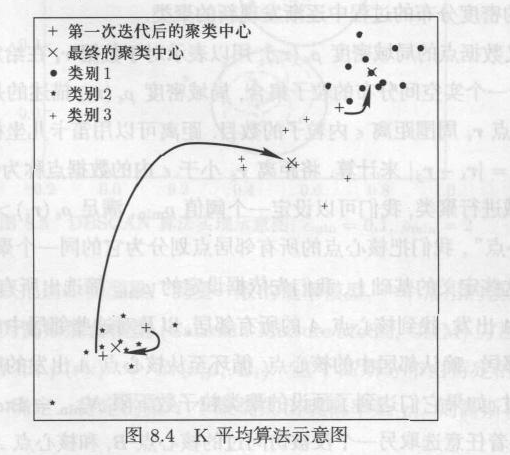
\includegraphics[width=0.58\linewidth]{figures/fig8_4_kmeans.png}
\caption{K 平均算法示意图}
\label{fig:kmeans}
\end{figure}

\begin{algorithmBox}[算法 8.2\quad K 平均聚类算法]
\begin{lstlisting}[style=bellacode]
function KMeans(X,K)
    centroids = InitializeCentroids(X,K)
    do
        Initialize clusters
        do x in X
            j = ArgMin_i(||x - centroids(i)||^2)
            clusters(j) = clusters(j) U x
        end
        do j = 1,K
            centroids(j) = Mean(clusters(j))
        end
    end while (centroids do not change)
    return clusters, centroids
end
\end{lstlisting}
\end{algorithmBox}

% R24 extends through source scan p.312 / printed p.297.

\originalpage{313}{298}
\subsubsection{密度聚类}
K 平均算法对于数据簇与数据簇之间区分明显的情况，效果较好。然而，如果数据分布不理想，K 平均算法会遇到一些困难，比较常见的情况是数据存在离群点或者数据特别稠密，都会导致 K 平均算法的收敛性变差，也就是上述的交叉迭代算法不能达到全局最优。

为解决这个问题，避免离散系数的迭代优化，我们不再预先设定聚类的数目，而是在探索数据的密度分布的过程中逐渐发现新的聚类。

首先定义数据点的局域密度 $\rho_\epsilon(r_i)$，用以表示对于数据 $r_i$ 在给定半径 $\epsilon$ 中的数据点个数。对于一个实空间分布的粒子集合，局域密度 $\rho_\epsilon(r_i)$ 描述的是真实的粒子数密度，也就是在点 $r_i$ 周围距离 $\epsilon$ 内粒子的数目。距离可以用笛卡儿坐标系下粒子之间的真实距离 $d_{ij}=|r_i-r_j|$ 来计算。将距离 $r_i$ 小于 $\epsilon$ 内的数据点称为邻居点。为了对密度较高的区域进行聚类，我们可以设定一个阈值 $\rho_{\min}$，满足 $\rho_\epsilon(r_i)>\rho_{\min}$ 的数据点 $r_i$ 定义为“核心点”，我们把核心点的所有邻居点划分为它的同一个聚类。

在以上这些定义的基础上，我们先依据设定的 $\rho_{\min}$ 筛选出所有核心点，再从任意的某核心点 $A$ 出发，找到核心点 $A$ 的所有邻居，以及对这些邻居中的所有核心点以同样的方式找邻居、确认邻居中的核心点，循环至从核心点 $A$ 出发的所有核心点及其邻居都被扫描过，如果它们达到了预设的聚类粒子数下限
\[
N_{\min}=\frac{4\pi}{3}\epsilon^3\rho,
\]
则它们组成一个聚类 $A$。接着任意选取另一个没被访问过的核心点 $B$，和核心点 $A$ 一样进行上述操作，得到另一个聚类 $B$。循环直至所有核心点都被访问，则完成聚类。
\jiaokan{印本将三维球半径 $\epsilon$ 内、数密度为 $\rho$ 时的期望粒子数写成 $4\pi\epsilon^3\rho$；若此处确实按球体积估算，应为 $(4\pi/3)\epsilon^3\rho$，故补入因子 $1/3$。DBSCAN 实际使用时的 MinPts 通常作为独立超参数给定。}

这种做法就是著名的 DBSCAN（Density-Based Spatial Clustering of Applications with Noise）算法，整个过程如图 8.5 所示，主要思想可以简述为由密度可达关系导出密度相连的样本集合，它具有的计算复杂度是 $O(N\log N)$。从直观上理解，DBSCAN 是基于密度的聚类方法，主要目标是将分布密度较高区域的数据归为一类，即寻找被低密度区域划分的高密度区域。

\subsubsection{概率聚类}
前面两种聚类方法理解起来比较直接，判断一个点是否属于某个聚类的时候只有是或者否。实际上，聚类也可以从贝叶斯统计出发，用概率模型的机器学习来理解。

假设某粒子 $r$ 在聚类 $i$ 的概率分布为条件概率 $p(r|i)$，第 $i$ 个聚类的出现概率是 $p_i$，满足 $\sum_i p_i=1$，则该粒子的总概率分布满足
\[
p(r)=\sum_i p(r|i)p_i.
\]
根据贝叶斯统计理论，一个粒子 $r$ 属于聚类 $i$ 的概率为
\[
p(i|r)=\frac{p(r|i)p_i}{\sum_j p(r|j)p_j}.
\]
其中条件概率 $p(r|i)$ 代表的就是一个概率模型，在 K 平均聚类方法中，可以认为这个概率模型是 $p(r|i)=\{0,1\}$，它由矩阵元素为 0 和 1 的系数矩阵确定。

\originalpage{314}{299}
\begin{figure}[htbp]
\centering
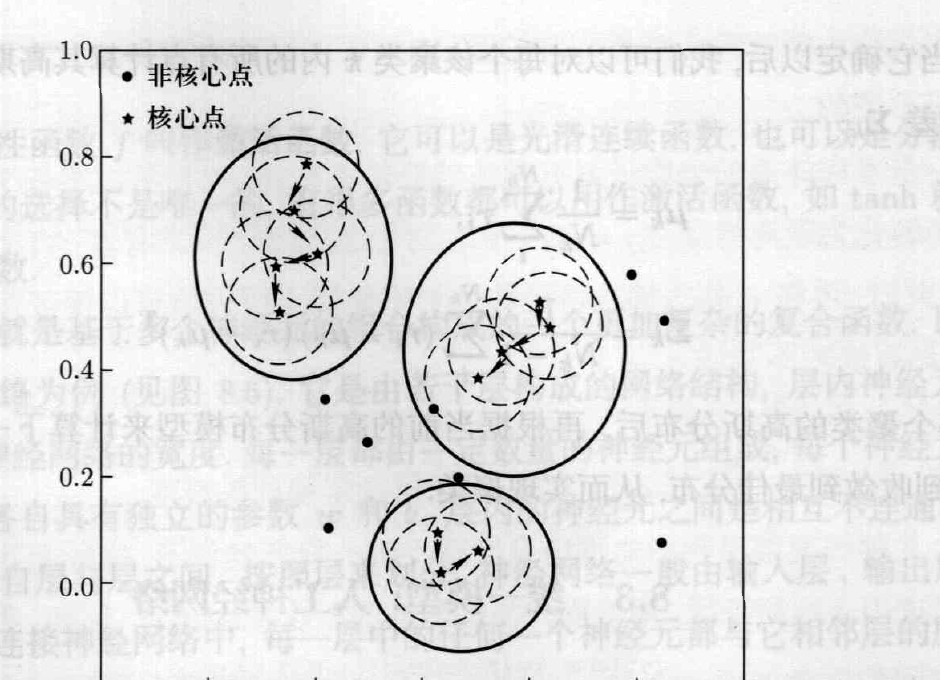
\includegraphics[width=0.58\linewidth]{figures/fig8_5_dbscan.png}
\caption{DBSCAN 算法实现示意图，$\epsilon_{\min}=0.1$，$\rho_{\min}=2$}
\label{fig:dbscan}
\end{figure}

显然，我们可以把这个模型推广到更一般的概率模型，一个常用的模型是基于高斯分布的模型，被称为高斯混合模型（Gaussian-Mixture Model, GMM）方法，即令 $p(r|i)$ 为一个多维高斯分布，$p(r|i)\sim N(r|\mu_i,\Sigma_i)$。这个高斯分布由待定的均值函数 $\mu_i$ 和协方差矩阵 $\Sigma_i$ 确定。待定的第 $i$ 个聚类的出现概率是 $p_i$，则高斯模型可以写为 $p(r|\mu_i,\Sigma_i,p_i)$。

对于一组数据集 $X=\{r^{(1)},r^{(2)},\ldots,r^{(M)}\}$，总的概率是
\begin{equation}
P\!\left(X\middle|\{\mu_i,\Sigma_i,p_i\}\right)=\prod_{k=1}^{M}p\!\left(r^{(k)}\middle|\mu_i,\Sigma_i,p_i\right).
\tag{8.2.13}
\end{equation}
模型可以在给定数据集 $X$ 的情况下通过求最大对数似然确定：
\begin{equation}
\theta_{\mathrm{opt}}=\{\mu_i,\Sigma_i,p_i\}_{\mathrm{opt}}:\quad
\max_{\{\mu_i,\Sigma_i,p_i\}}\ln P\!\left(X\middle|\{\mu_i,\Sigma_i,p_i\}\right).
\tag{8.2.14}
\end{equation}

与 K 平均聚类中一样，我们假定存在 $K$ 个聚类，$\sum_{k=1}^{K}p_k=1$。可以将 $p(r|\mu_i,\Sigma_i,p_i)$ 看成由两部分组成，一部分与 $N(r|\mu_i,\Sigma_i)$ 相关，它对应某个高斯函数模型，可以类比 K 平均聚类中定义的距离和给出的模型。另一部分描述的是在 $K$ 个高斯模型中选择出某一个的概率，可以类比 K 平均聚类中选择聚类的系数矩阵。

为了优化模型，可以采用迭代法，引入一个系数矩阵 $c_{ik}$，用它描述一个粒子 $i$ 是否属于高斯模型 $k$。对于第 $i$ 个粒子，列矢量 $c_i=\{0,\ldots,1,\ldots,0\}$，其中第 $k$ 个位置取 1，其余位置取 0，则认为粒子 $i$ 属于高斯模型 $k$。我们从一个初始猜测的 $c_{ik}$ 矩阵开始，当它确定以后，我们可以对每个该聚类 $k$ 内的所有点计算其高斯分布的均值 $\mu_k$ 和协方差 $\Sigma_k$：

\originalpage{315}{300}
\begin{equation}
\begin{aligned}
\mu_k&=\frac{1}{N_k}\sum_i^{N_k}r_i,\\
\Sigma_k&=\frac{1}{N_k}\sum_i^{N_k}(r_i-\mu_k)(r_i-\mu_k)^{\mathrm T}.
\end{aligned}
\tag{8.2.15}
\end{equation}
\jiaokan{印本式 (8.2.15) 的协方差归一化写为 $1/(N_k-1)$。前文明确以最大对数似然为优化目标时，高斯协方差的最大似然估计使用 $1/N_k$；$1/(N_k-1)$ 对应无偏样本协方差估计，并非该似然问题的极值解。此处按前文的最大似然语境改为 $1/N_k$。}
得到每个聚类的高斯分布后，再根据当前的高斯分布模型来计算下一步的聚类分布 $c_{ik}$，直到收敛到最佳分布，从而实现聚类。

\section{统一模型：人工神经网络}
在本章前面几节中，我们以回归问题为例讨论了监督式学习，以降维和聚类为例讨论了非监督式学习。总结起来，这些问题都可以归结为一个映射模型的训练，得到的映射关系就是所谓的机器学习模型。无论是哪一类问题，也无论是哪种学习模式，一个强大的算法的核心要求就是要有强大的表示能力，也就是能够表示待定的映射。因此，如果有一个表达能力强大且普适性高的机器学习模型框架，它可以被应用于以上各类问题的处理。人工神经网络，简称神经网络，就是这样一种框架。本节中我们将主要介绍全连接神经网络、卷积神经网络和受限玻尔兹曼机三种网络框架，并以全连接神经网络为例介绍其中比较关键的自动微分算法和梯度的网络参数优化算法。

\subsection{全连接神经网络}
\subsubsection{网络结构}
神经网络的基本单元是神经元。神经元在数学形式上可以被认为是一个广义的函数，对它输入一组特征值（自变量）就可以输出一个输出值，只不过这个“广义的函数”不是以一个孤立的解析函数的形式来描述，而是由一个线性函数和一个非线性函数组合而成的复合函数
\begin{equation}
y=f(w\cdot x+b)
\tag{8.3.1}
\end{equation}
来描述。

记输入的特征变量为 $x=(x_1,x_2,\ldots,x_d)$，首先通过一个线性运算得到一个标量值 $z$，
\begin{equation}
z=w\cdot x+b,
\tag{8.3.2}
\end{equation}
其中 $w$ 是一组系数，$b$ 是一个常数，它们都是神经网络模型中待确定的参数。上式中的输出值 $z$ 再通过一个非线性函数 $f$ 运算就可以得到另一个输出

\originalpage{316}{301}
\begin{equation}
y=f(z).
\tag{8.3.3}
\end{equation}
上式中的非线性函数 $f$ 叫作激活函数，它可以是光滑连续函数，也可以是分段光滑函数。激活函数的选择不是唯一的，有很多函数都可以用作激活函数，如 $\tanh$ 就是一种常用的激活函数。

神经网络就是基于多个神经元的组合构成的一个更加复杂的复合函数。以常见的全连接神经网络为例（见图 8.6），它是由若干层构成的网络结构，层内神经元的数目（$N_w$）被称为神经网络的宽度。每一层都由一定数量的神经元组成，每个神经元本身是相互独立的，各自具有独立的参数 $w$ 和 $b$。层内的神经元之间是相互不连通的，神经网络的连接来自层与层之间。按照层来划分，神经网络一般由输入层、输出层和隐藏层构成。在全连接神经网络中，每一层中的任何一个神经元都与它相邻层的所有神经元分别形成连接。

\begin{figure}[htbp]
\centering
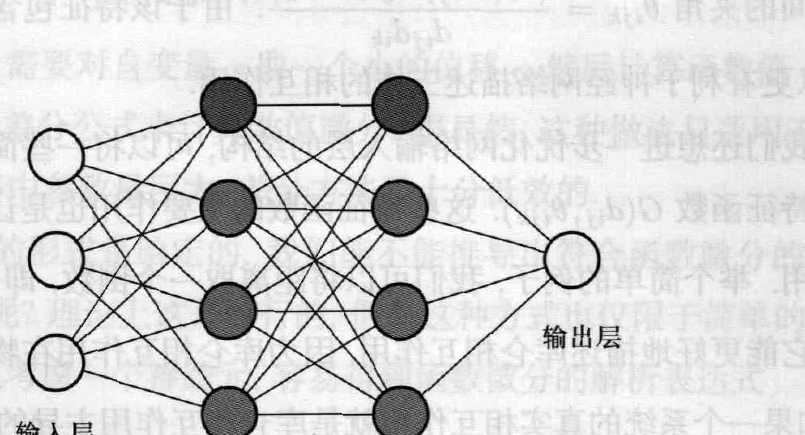
\includegraphics[width=0.60\linewidth]{figures/fig8_6_fcnn.png}
\caption{全连接神经网络结构示意图}
\label{fig:fcnn}
\end{figure}

神经网络中的输入层是直接与输入变量相连的一层，它起到的作用是把输入变量转化为一组能够在网络内部传递的隐变量：
\begin{equation}
a^0=F_{\mathrm{input}}(x_{\mathrm{input}}).
\tag{8.3.4}
\end{equation}
输入层中每个神经元可以写为 $a_j^0$，代表第 $j$ 个神经元的隐变量。

在应用神经网络时，输入层的设计至关重要，可以大大提高神经网络的表现或降低其训练难度。输入特征可以是一些独立的物理特征，也可以是物理特征的组合。我们以力场模型为例来展示输入特征设计的物理意义。令一个经典粒子体系的力场模型为 $V(r)$，粒子的位置坐标（位移矢量）$r=r_1,\ldots,r_N$ 是作为输入特征的一个自然选择。然而，这种做法并没有充分地利用好一个物理体系所具有的一些内禀的对称性和特征。

首先，在笛卡儿坐标系中势能 $V(r)$ 对所有粒子位置的整体平移是不变的。于是，我们可以引入一个质心位置，并计算出一组相对质心的位移矢量 $r_c=r-\frac1N\sum_i r_i$，然后再把它们作为新的输入变量传递给网络，就可以保证网络的输出随着所有粒子的整体平移是不变的。

\originalpage{317}{302}
进一步考虑体系的势能还具有整体的旋转不变性，我们可以将各个粒子的位移矢量进一步转化为距离特征 $d_{ij}=|r_i-r_j|$，对于 $N$ 个粒子，共存在 $N(N-1)/2$ 个距离特征 $d$。此时，再将 $d$ 作为输入特征传递给网络输入层后就可以保证输出的力场模型 $V(r)$ 也具有旋转不变性。

再进一步，如果一个待模拟的体系只有短程的相互作用，我们还可以对 $d_{ij}$ 特征进行截断，从而减少输入层的特征数，降低复杂度和训练难度。

以上几种情况都是利用物理信息来减少输入特征的例子，实际上我们也可以根据物理信息来引入新的特征，用于提升神经网络的有效表达能力。例如，我们可以引入三个粒子之间的夹角 $\theta_{ijk}$，
\[
\cos\theta_{ijk}=\frac{(r_i-r_j)\cdot(r_i-r_k)}{d_{ij}d_{ik}}.
\]
\jiaokan{印本直接写 $\theta_{ijk}=((r_i-r_j)\cdot(r_i-r_k))/(d_{ij}d_{ik})$，右端实际上是夹角的余弦，而非夹角本身。此处改写为 $\cos\theta_{ijk}=\cdots$；等价地也可写 $\theta_{ijk}=\arccos(\cdots)$。}
由于该特征包含了三个粒子之间的信息，它可以更有利于神经网络描述三体的相互作用。

如果我们还想进一步优化网络输入层的结构，可以将一些简单的输入特征放入预先设计的特征函数 $G(d_{ij},\theta_{ijk})$。这些特征函数的主要作用也是让网络更容易表达真实的相互作用。举个简单的例子，我们可以将距离取一个倒数，即令 $G(d_{ij})=1/d_{ij}$，那么可以预期它能更好地描述库仑相互作用，因为库仑势能在物理上反比于距离，而库仑力的大小反比于距离的平方。如果一个系统的真实相互作用就是库仑相互作用主导的，那么可以预期用 $1/d_{ij}$ 输入特征比直接用 $d_{ij}$ 得到的神经网络模型更准确。理论上，用 $d_{ij}$ 的线性和非线性函数的组合也可以表达 $1/d_{ij}$，但是这就意味着需要更多的网络参数。
\jiaokan{印本在以 $G(d_{ij})=1/d_{ij}$ 作为势能特征的同一段中写成“库仑相互作用反比于距离的平方”。若这里讨论的是势能 $V(r)$，库仑势能正比于 $1/r$；反比于 $r^2$ 的是库仑力的大小。正文据此区分二者。}

当变量由输入层传递给下一层网络后，变量 $a_k^l$ 开始在多层神经网络中进行传递，
\begin{equation}
a_j^{l+1}=f\left(\sum_k^{N_w}w_{jk}^{l}a_k^l+b_j^l\right).
\tag{8.3.5}
\end{equation}
下一层中某个神经元的变量依赖于上一层中的所有变量。这种网络层叫作隐藏层，它的层数称为深度神经网络的深度（$L$）。隐藏层中的神经元一般具有同样的结构，但是它们之间是相互独立的，具有不同的参数 $w_{jk}^l$ 和 $b_j^l$。神经网络的宽度越大、层数越多，其表达能力就越强，模型越精确，但是需要优化的参数也越多，优化难度越大，总体计算量越大。

在隐变量经过若干隐藏层的传递之后还需要一层输出层（$a^{L+1}$）将隐变量转化为输出变量：
\begin{equation}
y=F_{\mathrm{out}}(a^{L+1}).
\tag{8.3.6}
\end{equation}

\originalpage{318}{303}
输出层的宽度可以与隐藏层不同。对于力场模型的例子，我们可以将体系的总势能写为 $V_{\mathrm{total}}=\sum_{i=1}^{N}V_i$，其中 $V_i$ 为每个原子对总能量的贡献。每一项的能量 $V_i=F_{\mathrm{out}}(a^{L+1})$ 都可以从输出层引出一个输出变量来获得。

\subsubsection{自动微分}
神经网络的本质是一组复合函数。在神经网络的应用中，常常需要计算函数对自变量的导数。神经网络参数的优化也会需要计算损失函数对网络参数的导数。

我们先来看一看由单个神经元构成的复合函数的导数，记 $x$ 为输入，$y$ 为输出，神经元的非线性激活函数为 $f(x)=\tanh(x)$，线性项为 $g(x)=wx+b$。于是，单个神经元构成的复合函数为
\begin{equation}
y=f(g(x))=\tanh(wx+b).
\tag{8.3.7}
\end{equation}
如果采用数值差分法，需要对自变量 $x$ 取一个小的位移 $\epsilon$，然后计算函数值 $f(g(x+\epsilon))$ 或 $f(g(x-\epsilon))$，再通过差分公式来计算数值微分。很显然，这种做法只适用于参数比较少的情况，而神经网络中参数量巨大，差分方法是十分低效的。

既然神经元函数的形式是给定的，我们能不能推导出符合函数微分的解析形式，然后得到解析的微分呢？理论上这是可行的，但是这种方式也仅限于简单的复合函数。比如本例子中，如果只考虑一个神经元，容易得到函数微分的解析表达式
\begin{equation}
y'(x)=[1-\tanh^2(wx+b)]w.
\tag{8.3.8}
\end{equation}
再进一步考虑两个串联的神经元作为一个复合函数，
\begin{equation}
y=f_2(g_2(f_1(g_1(x))))=\tanh[w_2\tanh(w_1x+b_1)+b_2],
\tag{8.3.9}
\end{equation}
把它的微分的解析表达式写出来就已经是一个非常复杂的形式了：
\begin{equation}
y'(x)=w_1w_2[1-\tanh^2(w_2\tanh(w_1x+b_1)+b_2)][1-\tanh^2(w_1x+b_1)].
\tag{8.3.10}
\end{equation}
可以想象，当我们考虑大量神经元的网络时，解析表达式的复杂度会迅速变大，变得不具有计算可行性。

不过，神经网络中各个神经元具有确定的连接关系和解析性这两个特点让我们可以利用微分的链式法则。根据链式法则，神经元函数的导数可以写为如下连乘的形式：
\begin{equation}
y'(x)=f_2'(g_2(f_1(g_1(x))))\,g_2'(f_1(g_1(x)))\,f_1'(g_1(x))\,g_1'(x),
\tag{8.3.11}
\end{equation}
其中容易得到 $g_1'(x)=w_1$，然后可以计算 $f_1'(g_1(x))=1-\tanh^2(g_1(x))$，因为 $g_1(x)$ 是网络传递中需要计算的中间变量，因此将其直接代入 $f_1'$ 的解析公式即可。以此类推，可以计算得到 $y'(x)$。这就是自动微分。

\originalpage{319}{304}
可以看到，上述方式是在变量自输入层向输出层的传递过程中进行的导数计算，这种方式一般称为前向模式自动微分。由于每个神经元中的子函数都是相对简单的函数，可以得到其反函数的解析形式，那么也就容易得到导数的反向传递，一般称为反向模式自动微分。前向模式和反向模式是计算自动微分的两种主要模式。它们的适用情况主要取决于输入和输出的相对维度。设输入变量 $x$ 和输出变量 $y$ 的长度分别为 $M$ 和 $N$，以上讨论的微分 $dy/dx$ 可以表示为一个 $N\times M$ 的雅可比矩阵。在前向模式中，每完成一次自动微分可以获得所有中间变量对于一个自变量的导数，共需要 $M$ 次自动微分求导以得到完整的雅可比矩阵；在反向模式中，每完成一次自动微分可以获得一个因变量关于所有中间变量的导数，共需要 $N$ 次自动微分求导以得到完整的雅可比矩阵。在常见的机器学习模型中，一般都是输入的维度 $M$ 远远大于输出的维度 $N$，因此反向模式更加常用，其需要做的自动微分次数更少。实际上，很多的时候输出端的函数是一个值，$N=1$，这种情况下只需要一次自动微分就可以得到所有中间变量处的导数。

\subsubsection{网络参数优化}
有了上一小节的基础，我们以全连接神经网络模型的监督式学习为例讨论模型的训练。这个过程类似于前面介绍的回归问题。已知数据集为 $\{x_i,y_i\}$，网络的输出值（预测值）为 $\hat y_i(w)$。这里我们将所有参数简记为 $(w)$。网络参数优化的损失函数一般形式为
\begin{equation}
C(w)=\frac1N\sum_{i=1}^{N}[y_i-\hat y_i(w)]^2.
\tag{8.3.12}
\end{equation}
后续的优化过程就可以通过前面章节中介绍的优化算法进行。类似地，我们也可以在损失函数中加入合适的正则项来控制参数优化过程中同时需要满足的其他条件。

关于这些内容，前面的章节都有所讨论，本小节主要关注全连接神经网络中的梯度计算。因为很多的优化算法需要用到梯度的信息，所以是否能够高效地计算梯度至关重要。神经网络的结构复杂，变量和参数众多，一般都会采用上一小节所介绍的自动微分算法。上一小节中关于自动微分的介绍是基于函数对于自变量的导数展开的，而本小节中我们更加具体地给出损失函数关于网络参数的导数计算方法。

我们以全连接神经网络为例来看梯度在网络中的传递规律。我们用 $l=1,\ldots,L$ 标记层号，用 $w_{jk}^l$ 标记连接第 $l-1$ 层中第 $k$ 个神经元和第 $l$ 层中第 $j$ 个神经元的参数，偏移项记为 $b_j^l$。我们记中间网络第 $l$ 层第 $j$ 个特征为 $a_j^l$，同时再引入一个中间函数 $z_j^l$。对于变量的传递，我们把 $z_j^l$ 作为激活函数输入：
\begin{equation}
a_j^l=f(z_j^l),
\tag{8.3.13}
\end{equation}

\originalpage{320}{305}
从 $z_j^l$ 到 $a_j^l$ 是标量到标量。$z_j^l$ 由网络变量 $a_j^{l-1}$ 经过和待定参数 $w_{jk}^l$ 以及 $b_j^l$ 的线性运算得到，线性运算的表达式如下：
\begin{equation}
z_j^l=\sum_k w_{jk}^l a_k^{l-1}+b_j^l.
\tag{8.3.14}
\end{equation}
根据链式法则，由于 $a_j^l$ 和 $z_j^l$ 是由激活函数一对一连接起来的，所以有
\begin{equation}
\frac{\partial C}{\partial z_j^l}=\frac{\partial C}{\partial a_j^l}\frac{\partial a_j^l}{\partial z_j^l}.
\tag{8.3.15}
\end{equation}
定义 $f'(z_j^l)$ 为激活函数的微分：
\begin{equation}
f'(z_j^l)=\frac{\partial a_j^l}{\partial z_j^l}.
\tag{8.3.16}
\end{equation}
现在我们再来看损失函数对 $l$ 层的网络参数 $w_{jk}^l$ 和 $b_j^l$ 的梯度，因为优化是针对由 $w_{jk}^l$ 和 $b_j^l$ 组成的参数空间进行的。我们仅讨论 $w_{jk}^l$ 的情况，关于 $b_j^l$ 的情况类似且更简单。用中间变量 $z_j^l$ 展开梯度 $\partial C/\partial w_{jk}^l$ 的表达式，可得
\begin{equation}
\frac{\partial C}{\partial w_{jk}^l}=\frac{\partial C}{\partial z_j^l}\frac{\partial z_j^l}{\partial w_{jk}^l},
\tag{8.3.17}
\end{equation}
其中我们引入 $\Delta_j^l$ 定义第 $l$ 层第 $j$ 个神经元对于 $z_j^l$ 的梯度：
\begin{equation}
\Delta_j^l=\frac{\partial C}{\partial z_j^l},
\tag{8.3.18}
\end{equation}
且根据 $z_j^l$ 的表达式有 $\partial z_j^l/\partial w_{jk}^l=a_k^{l-1}$，因此损失函数对 $l$ 层的网络参数 $w_{jk}^l$ 求导的表达式可以写为如下形式：
\begin{equation}
\frac{\partial C}{\partial w_{jk}^l}=\Delta_j^l a_k^{l-1}.
\tag{8.3.19}
\end{equation}
于是，我们只需要计算每一层的传递变量 $\Delta_j^l$ 就可以通过一次简单的乘法获得对参数 $w_{jk}^l$ 的梯度。

接着，我们来看 $\Delta_j^l$ 在网络中的传递规律，为此我们尝试建立从 $\Delta_k^{l+1}$ 得到 $\Delta_j^l$ 的关系式。根据链式法则，我们可以得到如下推导：
\begin{equation}
\begin{aligned}
\Delta_j^l
&=\frac{\partial C}{\partial z_j^l}
=\sum_k\frac{\partial C}{\partial z_k^{l+1}}\frac{\partial z_k^{l+1}}{\partial z_j^l}\\
&=\left(\sum_k\Delta_k^{l+1}w_{kj}^{l+1}\right)f'(z_j^l).
\end{aligned}
\tag{8.3.20}
\end{equation}
\jiaokan{按式 (8.3.14) 的下标约定，$w_{jk}^l$ 的第一个下标对应当前层神经元、第二个下标对应前一层神经元。因此在由第 $l+1$ 层反传到第 $l$ 层时应出现 $w_{kj}^{l+1}$。印本式 (8.3.20) 写成 $w_{jk}^{l+1}$，下标次序与前文约定不一致，此处予以更正。}

\originalpage{321}{306}
这就是我们需要的一个梯度反向传递的关系。对于输出层，$z_j^L$ 是直接确定了损失函数的，所以可以直接得到损失函数 $C$ 对它的梯度：
\begin{equation}
\Delta_j^L=\frac{\partial C}{\partial z_j^L}.
\tag{8.3.21}
\end{equation}
以下是网络中反向传递计算的伪代码。

\begin{algorithmBox}[算法 8.3\quad 网络中反向传递计算]
\begin{lstlisting}[style=bellacode]
function back_propagation(L,w,b,x,y)
    a(0) = x
    do l = 1,L
        z(l) = w(l).a(l-1) + b(l)
        a(l) = f(z(l))
    end
    delta = C'(a(L),y) * f'(z(L))
    nabla_b(L) = delta
    nabla_w(L) = outer_product(delta,a(L-1))
    do l = L-1,1
        delta = transpose(w(l+1)).delta * f'(z(l))
        nabla_b(l) = delta
        nabla_w(l) = outer_product(delta,a(l-1))
    end
    return nabla_b,nabla_w
end
\end{lstlisting}
\end{algorithmBox}
\jiaokan{印本算法 8.3 的反向传播行写为 \texttt{delta = w(l+1).delta * f'(z(l))}。按式 (8.3.14) 的权重矩阵方向和式 (8.3.20) 的指标收缩，矩阵形式应使用下一层权重的转置，故改为 \texttt{transpose(w(l+1)).delta}。}

\subsection{卷积神经网络}
在上一小节的介绍中，我们提到了如何利用物理体系的一些对称性来设计全连接神经网络的输入特征。我们能不能有一种更加普适的方式来提取物理特征，从而设计出表示能力更强的网络结构呢？答案显然是可以且有必要的。

问题在于我们提取什么样的信息才是有效的？以经典力学系统为例，比如一个特定的结构（如由若干原子构成的一个分子），它应该具有平移对称性。另外，很多的系统还应该存在局域性，比如一个分子只是由相近的几个原子组成，远离该分子的其他原子不应该对这个分子的结构有很大的影响。同时，我们也应该考虑粒子之间存在的联系和相互作用，尤其是近邻的粒子之间的相互作用。要实现这样的信息提取，一个基本的数值运算就是卷积，它能够保持平移不变性和局域性特征。将卷积计算引入神经网络中就可以得到使用非常广泛的卷积神经网络。

\originalpage{322}{307}
具体地说，卷积神经网络的基本框架一般由卷积层（convolution）、池化层（pooling）和全连接层构成。实际上它与全连接神经网络的主要区别就是在进入全连接层之前先交替地进行卷积和池化操作。卷积层和池化层可以交替进行，最后再接到全连接网络，如图 8.7 所示。

\begin{figure}[htbp]
\centering
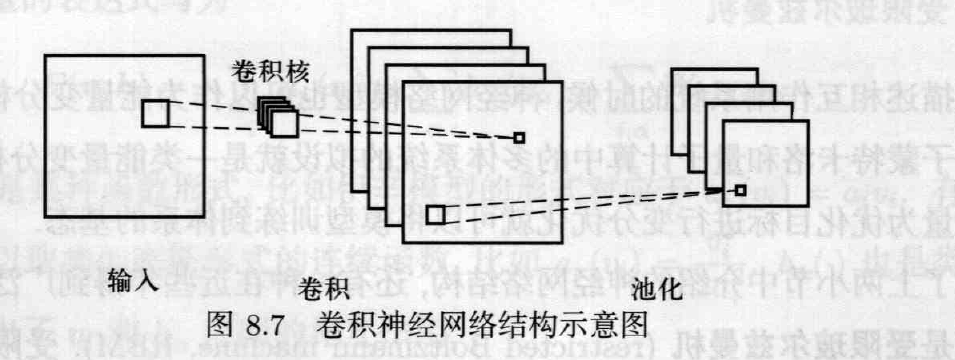
\includegraphics[width=0.70\linewidth]{figures/fig8_7_cnn.png}
\caption{卷积神经网络结构示意图}
\label{fig:cnn}
\end{figure}

卷积层的主要操作就是对输入的特征向量进行一个卷积计算。卷积计算由一个卷积核定义。我们以一维的数据矢量 $x(i)$，$i=1,\ldots,N$ 为例。我们构造一个卷积核 $h(j)$，$j=1,\ldots,M$，定义卷积后得到新的序列 $x_{\mathrm{new}}$ 仍具有长度 $N$：
\begin{equation}
x_{\mathrm{new}}(i)=[x*h]_i=\sum_{j=1}^{M}x(j)h(i-j).
\tag{8.3.22}
\end{equation}
\jiaokan{印本先定义卷积核 $h(j)$ 的指标范围为 $j=1,\ldots,M$，但式 (8.3.22) 的求和却写成 $j=0,\ldots,M$，会同时引入未定义的 $h(0)$ 并多出一个求和项。此处按前文的核指标约定改为 $j=1,\ldots,M$。}

在上面讨论的力场模型中，我们自然可以选取 $x(i)$ 为粒子的单粒子特征，比如单粒子的坐标，而卷积核可以选取为 $h(i-j)=W(r_i-r_j)$，其中令 $W$ 为待定的参数矩阵，它把单粒子坐标变量 $r_i$ 转化到长度为 $N$ 的新向量。卷积操作的结果实际上就是在单粒子变量的基础之上引入多粒子的依赖，用于描述相互作用，但是仍然在一定程度上保持其局域性。

总地来说，卷积层的数学形式可以写成下面这个表达式：
\begin{equation}
a_j^l=f\left(b_j^l+\sum_{i\in M_j}a_i^{l-1}*h_{ij}^l\right),
\tag{8.3.23}
\end{equation}
其中 $a_j^l$ 代表第 $l$ 层第 $j$ 个特征，$i$ 是前一层中的特征的指标，它属于与卷积核长度相等的第 $j$ 个卷积单元，$b_j^l$ 是第 $l$ 层第 $j$ 个卷积核的线性偏置，$h_{ij}^l$ 是第 $l$ 层第 $j$ 个卷积核中的第 $i$ 个元素，$f$ 是额外的非线性激活函数。

池化层是把多个元素依次组合以后减少输入特征的宽度的一层。以一维数据 $x(i)$，$i=1,\ldots,N$ 为例，设池化长度为 $N_p$，池化步长为 $N_s$，那么池化过程是将数列中的连续的 $N_p$ 个数组成一个数据池。第一个数据池从第一个数据开始，为 $\{x(1),x(2),\ldots,x(N_p)\}$；第二个数据池为从第 $1+N_s$ 个数据开始，为 $\{x(1+N_s),x(2+N_s),\ldots,x(N_p+N_s)\}$；以此类推，直至数据末尾，获得一系列数据池。

然后，我们再对该数据池定义一个操作，比如选择池内最大的数（最大值池化），或者对池内数据求和（求和池化），或者对池内数据取平均（平均池化）。选择完该数以后，把它传递给下一层的网络作为输入，那么下一层的输入数据量就等于数据池的数目，小于原本的数据量 $N$。从物理上看，池化其实就是粗粒化过程，用于进一步提取物理信息。

\originalpage{323}{308}
\subsection{受限玻尔兹曼机}
在描述相互作用系统的时候，神经网络模型也可以作为能量变分模型来使用。例如在量子蒙特卡洛和量子计算中的多体系统的拟设就是一类能量变分模型。将此类模型以能量为优化目标进行变分优化就可以将模型训练到体系的基态。

除了上两小节中介绍的神经网络结构，还有一种在近些年得到广泛关注的能量变分模型是受限玻尔兹曼机（restricted Boltzmann machine, RBM）。受限玻尔兹曼机的基本结构如图 8.8 所示，主要有两层，分别是输入层和隐藏层。输入层和隐藏层内部没有连接，但是输入层和隐藏层之间有连接。受限玻尔兹曼机的训练和优化等过程可以类比前两小节的介绍。因此，本小节主要讨论受限玻尔兹曼机作为能量变分模型的物理意义。

\begin{figure}[htbp]
\centering
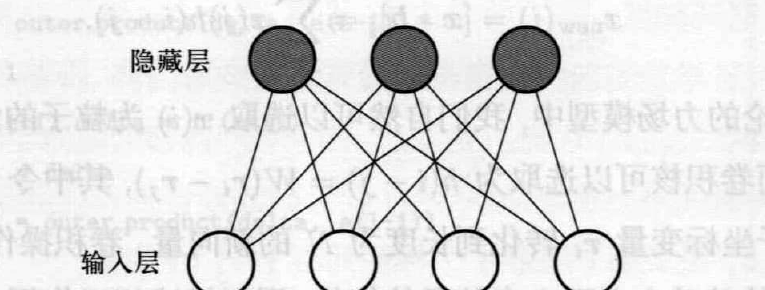
\includegraphics[width=0.52\linewidth]{figures/fig8_8_rbm.png}
\caption{受限玻尔兹曼机结构}
\label{fig:rbm}
\end{figure}

首先，我们以伊辛模型为例来看经典模型中相互作用是如何表达的，从而理解受限玻尔兹曼机中网络结构对于相互作用的表达：
\begin{equation}
E(v)=-\sum_i a_i v_i-\frac12\sum_{ij}v_iJ_{ij}v_j,
\tag{8.3.24}
\end{equation}
其中我们可以把 $v_i$ 当作描述每个点位状态的物理特征，比如格点模型上的自旋。$a_i$ 和 $J_{ij}$ 分别是模型参数。$a_i v_i$ 可以描述单个自旋在外场下的单体能量，$v_iJ_{ij}v_j$ 可以描述两个自旋状态之间的耦合。根据上述模型，伊辛模型的能量是特征 $v_i$ 的显式函数，给定一组 $v_i$ 就可以计算系统的能量。结合玻尔兹曼分布，就可以给出系统状态的经典统计分布 $p(v)$：
\begin{equation}
p(v)=\frac{e^{-E(v)}}{Z},
\tag{8.3.25}
\end{equation}
其中 $Z=\int e^{-E(v)}dv$ 是系统的配分函数。总地来说，在伊辛模型这样的经典模型中，相互作用是变量的显式表达式。

\originalpage{324}{309}
为了把受限玻尔兹曼机类比过来，我们可以用 $v_i$ 和 $h_\alpha$ 分别标记受限玻尔兹曼机输入层和隐藏层的特征，把输入层中的特征 $v_i$ 用于描述真实的物理特征，称为显变量（visible variable, $v$），隐藏层中的特征 $h_i$ 是无物理意义对应的潜变量（latent variable, $h$）。我们将能量的表达式写为
\begin{equation}
E(v,h)=-\sum_i a_i(v_i)-\sum_\alpha b_\alpha(h_\alpha)-\sum_{i,\alpha}W_{i\alpha}v_i h_\alpha.
\tag{8.3.26}
\end{equation}
$a_i(\cdot)$ 和 $b_\alpha(\cdot)$ 是某种函数形式，比如伊辛模型的形式对应于 $a_i(v_i)=a_i v_i$。有些情况下，$a_i(\cdot)$ 也可以取类似高斯形式的连续函数，比如 $a_i(v_i)=v_i^2/(2\sigma_i^2)$，$b_\alpha(\cdot)$ 也是类似的情况。$W_{i\alpha}$ 则给出了 $v_i$ 和 $h_\alpha$ 之间的相互作用。

可以看到，相比于伊辛模型中的相互作用是由 $v$ 和 $v$ 之间显式连接，受限玻尔兹曼机则是通过隐藏层 $h$ 和输入层 $v$ 之间的连接来间接地构造系统的相互作用。

下面我们来看物理变量 $v$ 之间的相互作用是如何通过潜变量的传播构造出来的。首先，显变量和潜变量构成的联合分布可以写为
\begin{equation}
p(v,h)=\frac{e^{-E(v,h)}}{Z},
\tag{8.3.27}
\end{equation}
进一步，对 $h$ 分量积分可以得到 $v$ 的分布
\begin{equation}
p(v)=\int\frac{e^{-E(v,h)}}{Z}\,dh.
\tag{8.3.28}
\end{equation}
同时，为了类比能量可以由显变量决定的经典模型，我们要求关于 $v$ 的分布满足经典统计分布
\begin{equation}
p(v)=\frac{e^{-E(v)}}{Z}.
\tag{8.3.29}
\end{equation}
联合上述关系可以得到
\begin{equation}
\begin{aligned}
E(v)&=-\ln\int dh\,e^{-E(v,h)}\\
&=-\sum_i a_i(v_i)-\sum_\alpha\ln\int e^{b_\alpha(h_\alpha)+\sum_i v_iW_{i\alpha}h_\alpha}\,dh_\alpha.
\end{aligned}
\tag{8.3.30}
\end{equation}

关于潜变量，我们可以定义它的分布
\begin{equation}
q_\alpha(h_\alpha)=\frac{e^{b_\alpha(h_\alpha)}}{Z_\alpha},\qquad Z_\alpha=\int e^{b_\alpha(h_\alpha)}\,dh_\alpha.
\tag{8.3.31}
\end{equation}
\jiaokan{印本式 (8.3.31) 将单个潜变量的归一化分母写成系统总配分函数 $Z$。为了使 $q_\alpha$ 本身成为归一化概率分布，其分母应是对应单变量分布的归一化常数 $Z_\alpha=\int e^{b_\alpha(h_\alpha)}dh_\alpha$，故予以更正。}
再定义一个累积量生成函数
\begin{equation}
K_\alpha(t)=\ln\int q_\alpha(h_\alpha)e^{h_\alpha t}\,dh_\alpha
=\sum_n\kappa_\alpha^{(n)}\frac{t^n}{n!},\qquad
\kappa_\alpha^{(n)}=\left.\partial_t^n K_\alpha(t)\right|_{t=0}.
\tag{8.3.32}
\end{equation}

\originalpage{325}{310}
用累积量生成函数可以将能量表达式改写为
\begin{equation}
\begin{aligned}
E(v)
&=-\sum_i a_i(v_i)-\sum_\alpha K_\alpha\!\left(\sum_iW_{i\alpha}v_i\right)\\
&=-\sum_i a_i(v_i)-\sum_\alpha\sum_n\kappa_\alpha^{(n)}
\frac{\left(\sum_iW_{i\alpha}v_i\right)^n}{n!}\\
&=-\sum_i a_i(v_i)-\sum_i\left(\sum_\alpha\kappa_\alpha^{(1)}W_{i\alpha}\right)v_i
-\frac12\sum_{ij}\left(\sum_\alpha\kappa_\alpha^{(2)}W_{i\alpha}W_{j\alpha}\right)v_iv_j+\cdots.
\end{aligned}
\tag{8.3.33}
\end{equation}
从上式中不难看出通过隐藏层引入潜变量后可以描述输入层内显变量之间的高阶相互作用。

受限玻尔兹曼机可以进一步拓展成深度玻尔兹曼机，也就是具有多个隐藏层的玻尔兹曼机，可以进一步拓展玻尔兹曼机网络的表达能力，也就是模型对于变量之间的相互作用的表示能力。

\subsection{霍普菲尔德网络}
霍普菲尔德（Hopfield）网络是另一种特殊的神经网络，也是基于物理系统的能量变分原理来对网络进行优化。它在神经网络的早期研究中也具有很重要的历史地位，尤其是对于理解大脑和神经网络中记忆的形成具有重要的作用。在计算机中，需要知道数据在内存中的确切地址才能获取对应的数据。而人类大脑中的记忆是通过联想的方法来获取的。例如，看见一个特定的物体，会回想起与之关联的事情；对于经历过但记不清的事情，经过别人的提醒可以较清楚地回忆起来。事实上，物理系统也可以有记忆。例如，弹簧由平衡状态经过有限的形变之后依然能够回到初态，也可以视为弹簧具有对初态的记忆。

作为一个简单的例子，我们考虑一个推广的零场伊辛模型，每个格点的自旋 $s_i=\pm1$。对于自旋构型 $S=(s_1,s_2,\ldots,s_n)$，系统的哈密顿量可以表示为
\begin{equation}
H[S]=-\sum_{i\ne j}J_{ij}s_i s_j.
\tag{8.3.34}
\end{equation}
其中 $J_{ij}$ 表示 $i$ 格点和 $j$ 格点自旋的耦合强度。当所有近邻格点 $(i,j)$ 间的耦合强度为一个常数且非近邻格点间无耦合时，这个模型就退化到普通的铁磁伊辛模型。如果让系统朝着能量最小化的方向演化，那么系统会倾向于形成铁磁态，即 $s_i=1$ 或 $s_i=-1$，但具体收敛到哪个态与初态有关。可以认为该模型体系具有铁磁态的记忆，系统从一个不规则的初态朝能量极小值处演化的过程也可以被视为记忆联想过程。如果考虑更一般的情形，即让每个 $J_{ij}$ 的取值不同，这就对应了一个自旋玻璃体系，系统会具有更复杂的记忆。

\footnote{霍普菲尔德因对利用神经网络实现机器学习的基础性贡献，与辛顿（Hinton）一起获得了 2024 年度诺贝尔物理学奖。}

\originalpage{326}{311}
受此启发，为了更好地研究记忆过程，可以将自旋玻璃系统抽象为一个简单的网络，这就是霍普菲尔德网络。该网络没有一般意义上的输入层和输出层，它的输入和输出分别为初态和末态。网络由 $n$ 个神经元组成，每个神经元都具有一个值 $x_i=\pm1$（见图 8.9）。每对神经元 $i,j$ 之间存在双向连接，每个连接都具有权重 $w_{ij}$，并且 $w_{ij}=w_{ji}$，还规定每个神经元没有自相互作用，即 $w_{ii}=0$。霍普菲尔德网络对应的能量函数可以表示为
\begin{equation}
E=-\frac12\sum_{i,j}w_{ij}x_i x_j.
\tag{8.3.35}
\end{equation}
\jiaokan{印本式 (8.3.35) 在对称权重 $w_{ij}=w_{ji}$ 且对 $i,j$ 双重求和的约定下漏写了因子 $1/2$。标准 Hopfield 能量为 $E=-\frac12\sum_{ij}w_{ij}x_ix_j$（若只对无序对 $i<j$ 求和则可不写 $1/2$）。此处按印本后文的双重求和记号补入。}

对能量的最小化过程可通过一系列随机的演化过程来实现。我们将每一步的演化定义为离散的时间步。在每个时间步中，一个随机的神经元会被选中，并按照如下规则更新：
\begin{equation}
x_i^{(t+1)}=f\left(\sum_j w_{ij}x_j^{(t)}\right),
\tag{8.3.36}
\end{equation}
其中 $f$ 为激活函数，满足
\begin{equation}
f(y)=\begin{cases}
1,& y\ge0,\\
-1,& y<0.
\end{cases}
\tag{8.3.37}
\end{equation}
这意味着，如果改变当前神经元的状态 $x_i$ 能够使得总能量降低，那就进行改变。于是在每个时间步之后，霍普菲尔德网络的能量都会降低或保持不变。在经过足够多时间步的演化之后，网络会收敛到某个能量极小值点，这个能量极小值点就对应了霍普菲尔德网络的记忆，网络的演化过程就对应了记忆的联想过程。

\begin{figure}[htbp]
\centering
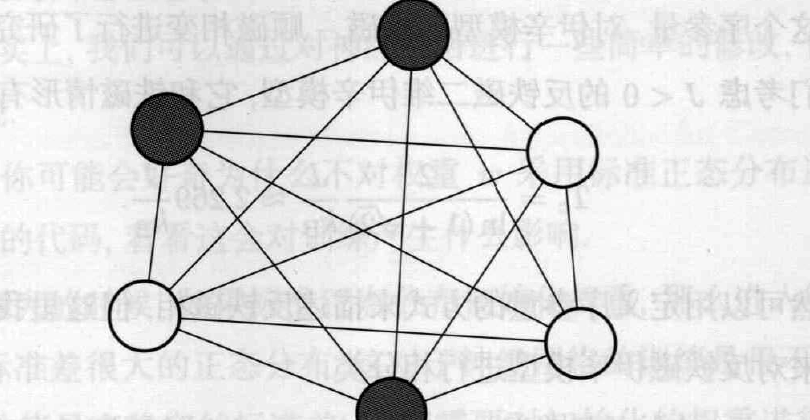
\includegraphics[width=0.48\linewidth]{figures/fig8_9_hopfield.png}
\caption{包含 6 个神经元的霍普菲尔德网络结构示意图}
\label{fig:hopfield}
\end{figure}

\originalpage{327}{312}
霍普菲尔德网络的能量函数是由网络超参数 $w_{ij}$ 的取值决定的，极小值点的位置也与其取值有关。我们可以让 $w_{ij}$ 取一些特定的值，从而控制能量的极小值点，让网络具有特定的记忆。例如，为了让网络具有 $V=(v_1,v_2,\ldots,v_n)$ 的记忆，可以取 $w_{ij}=v_iv_j$，此时 $x_i=v_i$ 显然为能量的极小值点。此外，霍普菲尔德网络还可以存储多个无关联的记忆。用 $p$ 标记不同的记忆，只需要将不同记忆对应的能量函数叠加，即取
\begin{equation}
w_{ij}=\sum_p v_i^p v_j^p,
\tag{8.3.38}
\end{equation}
就能够让能量函数具有多个特定的极小值，从而具有多个记忆。然而，对于给定大小的霍普菲尔德网络，当其存储的记忆足够多时，不同的能量函数之间会相互影响，甚至使原本的极小值点不复存在，或者出现新的极小值点。因此，霍普菲尔德网络能够稳定存储的记忆是有限的。可以证明，上述霍普菲尔德网络能够稳定存储的记忆与神经元的数量成线性关系。考虑到实际的机器学习任务往往需要处理并记忆数据中的大量模式，随神经元数线性增长的记忆能力是难以接受的。为此，可以通过引入其他能量函数等方法，进一步提升霍普菲尔德网络的记忆存储容量。

\begin{exerciseBox}[大作业：反铁磁二维伊辛模型相分类]
我们在之前统计物理的章节中，以伊辛模型为例对相变和临界现象进行了研究。通过蒙特卡洛采样的方法，我们可以得到一系列在不同温度下的自旋构型 $S=(s_1,s_2,\ldots,s_n)$。在零场的情况下，哈密顿量为
\begin{equation}
H[S]=-J\sum_{\langle i,j\rangle}s_i s_j,
\tag{1}
\end{equation}
其中 $\langle i,j\rangle$ 表示相邻的自旋对。在之前的章节中，我们研究了 $J>0$ 的铁磁情形，并利用平均自旋这个序参量，对伊辛模型的铁磁--顺磁相变进行了研究。

现在我们考虑 $J<0$ 的反铁磁二维伊辛模型，它和铁磁情形有着相同的临界温度
\begin{equation}
T_c=\frac{2}{\ln(1+\sqrt2)}\frac{|J|}{k_{\mathrm B}}\approx2.269\frac{|J|}{k_{\mathrm B}}.
\tag{2}
\end{equation}
\jiaokan{印本在明确设定 $J<0$ 的反铁磁模型后仍写成 $T_c\propto J$，会给出负的临界温度。二维方格 Ising 模型的临界温度取决于耦合强度的绝对值，故改为 $|J|$。}
尽管我们依然可以用定义序参量的方式来描述反铁磁相，但这里我们将训练一个简单的神经网络来对反铁磁伊辛模型进行相分类。

1. 取 $J=-1$，玻尔兹曼常数 $k_{\mathrm B}=1$，在 $30\times30$ 的周期性正方格点上，利用局部更新方法分别生成相变温度以下和相变温度以上的构型数据集。
\end{exerciseBox}

\originalpage{328}{313}
\begin{exerciseBox}[大作业（续）]
作为参考，你可以在不同的温度下，总共生成 10000 个自旋构型。为简单起见，这里不考虑马尔可夫链是否达到稳定，你可以从随机的自旋构型出发，在 50000 次迭代之后，每隔 5000 步取一个构型。

2. 按照以下提示，从头实现并训练一个简单的神经网络，对高温相和低温相的自旋构型进行分类。

你可以将网络的输入维度设为 $30\times30=900$，输出维度为 1，中间只有一层大小为 36 的隐藏层。网络的输出 $y$ 满足 $0<y<1$，其中 $y<0.5$ 表示网络判断输入构型为低温相，反之则为高温相。对所有的权重 $w$ 在初始化时置为 0，所有偏置 $b$ 采用标准正态分布的方式进行初始化。神经网络的激活函数选用 Sigmoid 函数 $\sigma(x)=(1+e^{-x})^{-1}$。

对于网络的训练，可以根据本章中给出的梯度反向传播公式，使用平方损失函数作为成本函数进行优化。在优化的过程中，如果计算所有构型后得到总的成本函数，再根据其对于参数的导数进行梯度下降，那么一次参数更新就需要巨大的计算量。然而计算全部与计算一小部分构型得到的成本函数及其关于参数的导数，对于参数的更新来说并没有很大的区别。于是我们可以采用小批量（mini batch）更新的方法，比如在一轮（epoch）参数更新中，把 10000 个数据分成 100 份，每次只取一份中的 100 个自旋构型计算成本函数并优化参数，这样能以更小的计算量进行更多次的迭代，加速网络的收敛。
\jiaokan{印本前文要求“总共生成 10000 个自旋构型”，此处却写成“把 100000 个数据分成 100 份”，与紧接着“每份 100 个”也不一致。$10000/100=100$，故按全段数据规模改为 10000。}
作为参考，如果每个小批量包含 100 个自旋构型，那么每次参数更新 $w'=w-\eta\,\partial V/\partial w$ 时，学习率 $\eta$ 可以取为 0.01。

为了更好地看到网络的训练效果，我们还需要在训练的每一步输出神经网络判断的准确率。尽管我们可以直接输出网络在训练集上的准确率，但这不利于我们及时发现网络的过拟合倾向：网络可能在训练数据集上表现不错，但对没有见过的数据却无法给出准确的判断。所以更好的做法是把数据集分成训练数据集和验证数据集，每步输出网络在验证数据集上的准确率。

3. 尽管相分类的问题看起来很简单，我们在上一问中实现的神经网络的表现却似乎不尽如人意。事实上，我们可以通过对神经网络进行一些简单的修改，使它在这个问题上有更好的表现。

在上一问中，你可能会好奇为什么不对权重 $w$ 采用标准正态分布进行随机初始化。尝试改动相关的代码，看看这会对训练产生什么影响。

当输入维度很大的时候，如果标准正态分布初始化权重，那么进入第一个隐藏层的数值会是一个标准差很大的正态分布。这对于神经网络的训练是很不利的。为了保证传入下一层的数值具有稳定的标准差，我们需要对初始化的权重进行一定的处理。具体来说，对于输入维度为 900 的情况，我们应该在标准正态分布的基础上除以 30 作为初始化的权重。尝试修改初始化部分的代码，相比于直接采用标准正态分布，它能带来多大的效果？
\end{exerciseBox}

\originalpage{329}{314}
\begin{exerciseBox}[大作业（续）]
除此之外，对于伊辛模型这个特定的问题，我们知道序参量为零代表了顺磁相，非零代表反铁磁相。然而 Sigmoid 激活函数不能很好地利用到这一性质，限制了网络在这个问题上的表达能力。在优化过权重初始化的基础上，改动代码把第一层网络的激活函数换成 $\operatorname{ReLU}(x)=\max(0,x)$，观察它相比于 Sigmoid 函数给神经网络准确率带来的提升。

4. 使用主成分分析，找出所有训练构型中的两个主成分，并绘制散点图。图中用不同颜色的点标记高温相和低温相。体会主成分分析在这个问题中相比于神经网络的优势与局限性。
\end{exerciseBox}

% R25 completes source scan pp.313--329 / printed pp.298--314.
